% Options for packages loaded elsewhere
% Options for packages loaded elsewhere
\PassOptionsToPackage{unicode}{hyperref}
\PassOptionsToPackage{hyphens}{url}
\PassOptionsToPackage{dvipsnames,svgnames,x11names}{xcolor}
%
\documentclass[
  letterpaper,
  DIV=11,
  numbers=noendperiod]{scrartcl}
\usepackage{xcolor}
\usepackage{amsmath,amssymb}
\setcounter{secnumdepth}{5}
\usepackage{iftex}
\ifPDFTeX
  \usepackage[T1]{fontenc}
  \usepackage[utf8]{inputenc}
  \usepackage{textcomp} % provide euro and other symbols
\else % if luatex or xetex
  \usepackage{unicode-math} % this also loads fontspec
  \defaultfontfeatures{Scale=MatchLowercase}
  \defaultfontfeatures[\rmfamily]{Ligatures=TeX,Scale=1}
\fi
\usepackage{lmodern}
\ifPDFTeX\else
  % xetex/luatex font selection
\fi
% Use upquote if available, for straight quotes in verbatim environments
\IfFileExists{upquote.sty}{\usepackage{upquote}}{}
\IfFileExists{microtype.sty}{% use microtype if available
  \usepackage[]{microtype}
  \UseMicrotypeSet[protrusion]{basicmath} % disable protrusion for tt fonts
}{}
\makeatletter
\@ifundefined{KOMAClassName}{% if non-KOMA class
  \IfFileExists{parskip.sty}{%
    \usepackage{parskip}
  }{% else
    \setlength{\parindent}{0pt}
    \setlength{\parskip}{6pt plus 2pt minus 1pt}}
}{% if KOMA class
  \KOMAoptions{parskip=half}}
\makeatother
% Make \paragraph and \subparagraph free-standing
\makeatletter
\ifx\paragraph\undefined\else
  \let\oldparagraph\paragraph
  \renewcommand{\paragraph}{
    \@ifstar
      \xxxParagraphStar
      \xxxParagraphNoStar
  }
  \newcommand{\xxxParagraphStar}[1]{\oldparagraph*{#1}\mbox{}}
  \newcommand{\xxxParagraphNoStar}[1]{\oldparagraph{#1}\mbox{}}
\fi
\ifx\subparagraph\undefined\else
  \let\oldsubparagraph\subparagraph
  \renewcommand{\subparagraph}{
    \@ifstar
      \xxxSubParagraphStar
      \xxxSubParagraphNoStar
  }
  \newcommand{\xxxSubParagraphStar}[1]{\oldsubparagraph*{#1}\mbox{}}
  \newcommand{\xxxSubParagraphNoStar}[1]{\oldsubparagraph{#1}\mbox{}}
\fi
\makeatother


\usepackage{longtable,booktabs,array}
\usepackage{calc} % for calculating minipage widths
% Correct order of tables after \paragraph or \subparagraph
\usepackage{etoolbox}
\makeatletter
\patchcmd\longtable{\par}{\if@noskipsec\mbox{}\fi\par}{}{}
\makeatother
% Allow footnotes in longtable head/foot
\IfFileExists{footnotehyper.sty}{\usepackage{footnotehyper}}{\usepackage{footnote}}
\makesavenoteenv{longtable}
\usepackage{graphicx}
\makeatletter
\newsavebox\pandoc@box
\newcommand*\pandocbounded[1]{% scales image to fit in text height/width
  \sbox\pandoc@box{#1}%
  \Gscale@div\@tempa{\textheight}{\dimexpr\ht\pandoc@box+\dp\pandoc@box\relax}%
  \Gscale@div\@tempb{\linewidth}{\wd\pandoc@box}%
  \ifdim\@tempb\p@<\@tempa\p@\let\@tempa\@tempb\fi% select the smaller of both
  \ifdim\@tempa\p@<\p@\scalebox{\@tempa}{\usebox\pandoc@box}%
  \else\usebox{\pandoc@box}%
  \fi%
}
% Set default figure placement to htbp
\def\fps@figure{htbp}
\makeatother





\setlength{\emergencystretch}{3em} % prevent overfull lines

\providecommand{\tightlist}{%
  \setlength{\itemsep}{0pt}\setlength{\parskip}{0pt}}



 


\KOMAoption{captions}{tableheading}
\makeatletter
\@ifpackageloaded{caption}{}{\usepackage{caption}}
\AtBeginDocument{%
\ifdefined\contentsname
  \renewcommand*\contentsname{Table of contents}
\else
  \newcommand\contentsname{Table of contents}
\fi
\ifdefined\listfigurename
  \renewcommand*\listfigurename{List of Figures}
\else
  \newcommand\listfigurename{List of Figures}
\fi
\ifdefined\listtablename
  \renewcommand*\listtablename{List of Tables}
\else
  \newcommand\listtablename{List of Tables}
\fi
\ifdefined\figurename
  \renewcommand*\figurename{Figure}
\else
  \newcommand\figurename{Figure}
\fi
\ifdefined\tablename
  \renewcommand*\tablename{Table}
\else
  \newcommand\tablename{Table}
\fi
}
\@ifpackageloaded{float}{}{\usepackage{float}}
\floatstyle{ruled}
\@ifundefined{c@chapter}{\newfloat{codelisting}{h}{lop}}{\newfloat{codelisting}{h}{lop}[chapter]}
\floatname{codelisting}{Listing}
\newcommand*\listoflistings{\listof{codelisting}{List of Listings}}
\makeatother
\makeatletter
\makeatother
\makeatletter
\@ifpackageloaded{caption}{}{\usepackage{caption}}
\@ifpackageloaded{subcaption}{}{\usepackage{subcaption}}
\makeatother
\usepackage{bookmark}
\IfFileExists{xurl.sty}{\usepackage{xurl}}{} % add URL line breaks if available
\urlstyle{same}
\hypersetup{
  pdftitle={Theoretical Background: Radar Remote Sensing Fundamentals},
  pdfauthor={David Moravec},
  colorlinks=true,
  linkcolor={blue},
  filecolor={Maroon},
  citecolor={Blue},
  urlcolor={Blue},
  pdfcreator={LaTeX via pandoc}}


\title{Theoretical Background: Radar Remote Sensing Fundamentals}
\author{David Moravec}
\date{2025-12-12}
\begin{document}
\maketitle

\renewcommand*\contentsname{Table of contents}
{
\hypersetup{linkcolor=}
\setcounter{tocdepth}{3}
\tableofcontents
}

\section{Introduction: The Active Microwave
Perspective}\label{introduction-the-active-microwave-perspective}

Radar (Radio Detection and Ranging) remote sensing represents a
fundamentally different approach to Earth observation compared to
optical and infrared methods. While passive optical sensors rely on
reflected sunlight, radar systems actively transmit microwave radiation
and measure the backscattered signal (\textbf{lillesand2015remote?}).
This active nature, combined with the long wavelengths of microwave
radiation (ranging from millimeters to meters), provides unique
capabilities that overcome many limitations of passive optical remote
sensing.

The electromagnetic spectrum shows that microwave radiation occupies the
region between radio waves and infrared radiation, with wavelengths
ranging from approximately 1 mm to 1 m (Figure~\ref{fig-em-spectrum}).
Within the atmosphere, specific wavelength regions---called atmospheric
windows---allow electromagnetic radiation to propagate with minimal
attenuation. The microwave region features broad atmospheric windows
that enable radar signals to penetrate clouds, fog, rain, and darkness,
providing all-weather, day-and-night imaging capabilities
(\textbf{ulaby2014microwave?}).

\begin{figure}

\centering{

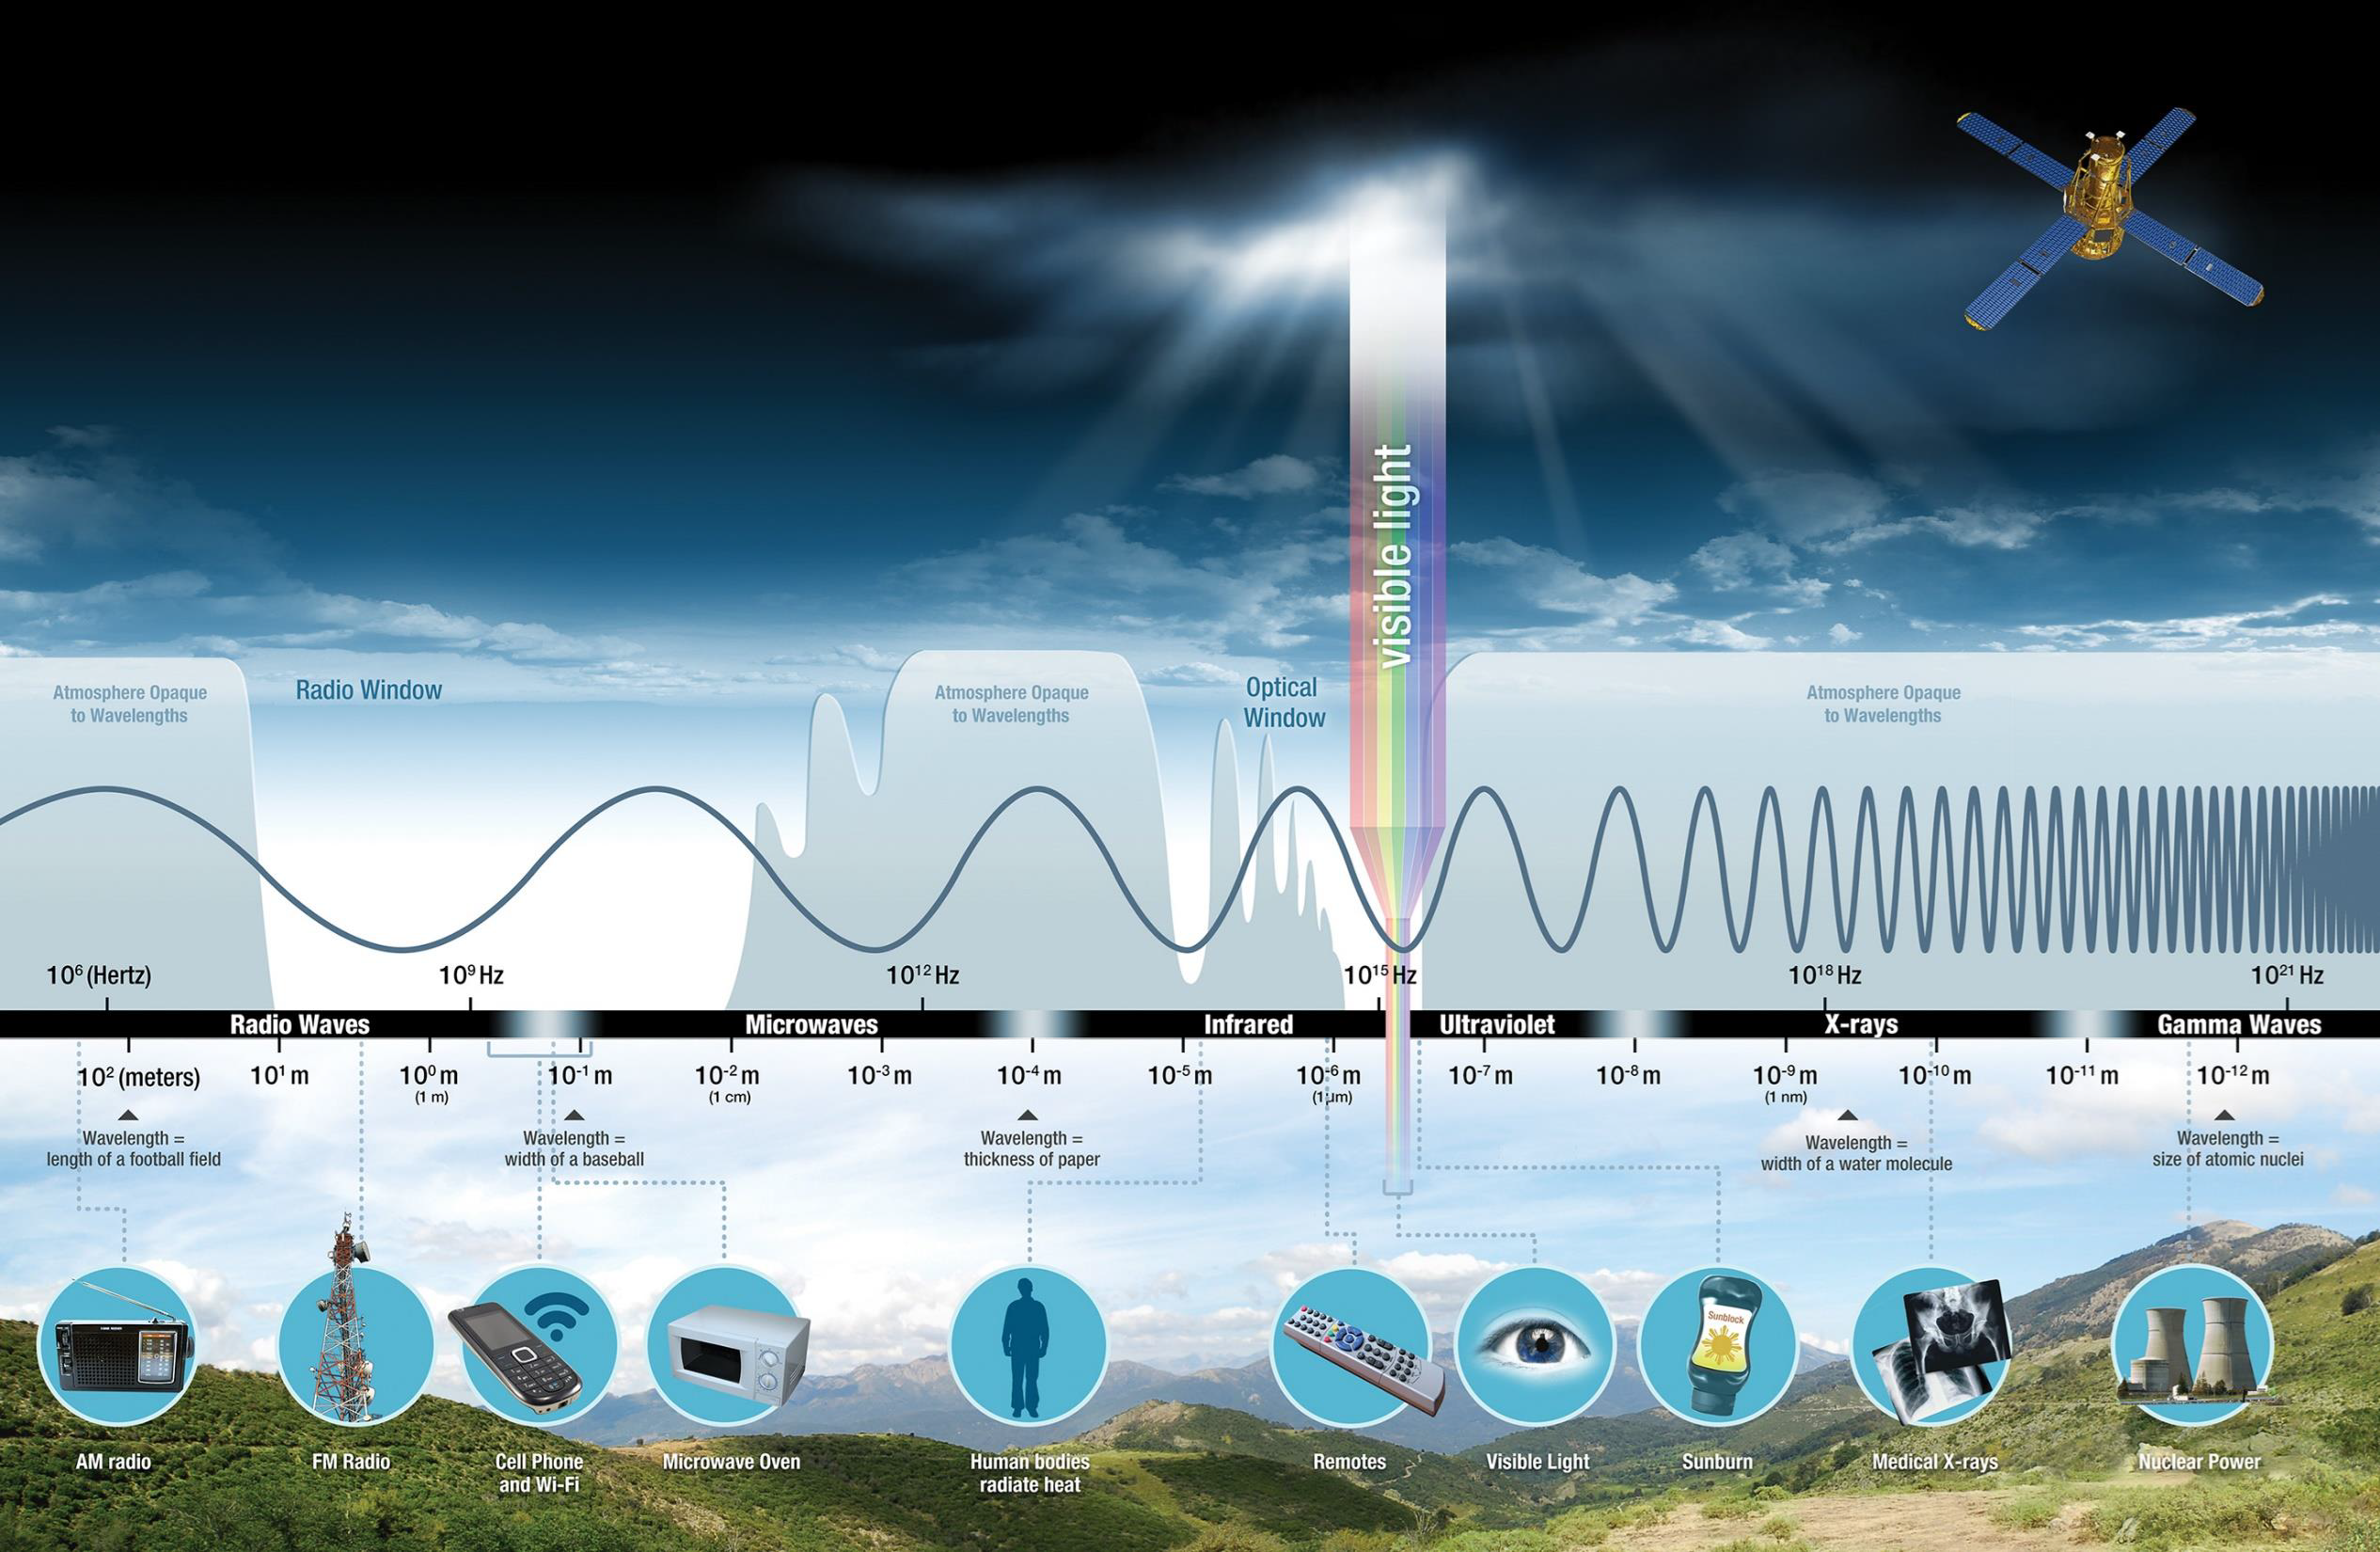
\includegraphics[width=1\linewidth,height=\textheight,keepaspectratio]{RADAR_figures/em_spectrum.png}

}

\caption{\label{fig-em-spectrum}Electromagnetic spectrum showing the
position of radar bands. The microwave region (highlighted) spans
wavelengths from \textasciitilde1 mm to 1 m, corresponding to
frequencies from 300 GHz to 300 MHz. Common radar bands are labeled: Ka,
K, Ku, X, C, S, L, and P-band. The lower graph shows atmospheric
opacity, with the microwave ``radio window'' demonstrating excellent
atmospheric transmission compared to visible and infrared regions.}

\end{figure}%

Three fundamental advantages distinguish radar from optical remote
sensing:

\begin{enumerate}
\def\labelenumi{\arabic{enumi}.}
\tightlist
\item
  \textbf{Active illumination}: Radar provides its own energy source,
  enabling observations regardless of solar illumination and at any time
  of day or night (\textbf{henderson2998manual?})
\item
  \textbf{Cloud penetration}: Microwave radiation passes through clouds,
  smoke, and atmospheric moisture that block optical sensors
  (\textbf{woodhouse2017introduction?})
\item
  \textbf{Surface penetration}: Longer radar wavelengths can penetrate
  vegetation canopies and even soil or ice surfaces, revealing
  subsurface structures and volume properties
  (\textbf{ulaby2014microwave?})
\end{enumerate}

These capabilities make radar particularly valuable for forest
monitoring, where cloud cover often obscures optical observations in
tropical and temperate regions, and where information about forest
structure extends throughout the three-dimensional canopy volume rather
than just the top surface visible to optical sensors.

\section{The Importance of Forests: Context for Radar
Applications}\label{the-importance-of-forests-context-for-radar-applications}

Understanding why radar remote sensing matters for forest monitoring
requires first appreciating the critical role forests play in Earth's
systems (Figure~\ref{fig-forest-importance}). Forests are crucial for
regulating energy, water, and carbon balance, covering 31\% of Earth's
solid surface and 43\% of the European Union's area
(\textbf{bonan2008forests?}). They represent Europe's most important
renewable source of biomass and deliver livelihoods for 1.6 billion
people globally (\textbf{fao2020?}). Forests provide habitat for the
vast majority of terrestrial plant and animal species, making their
monitoring essential for biodiversity conservation
(\textbf{fao2020state?}).

\begin{figure}

\centering{

\includegraphics[width=1\linewidth,height=\textheight,keepaspectratio]{RADAR_figures/forest_importance.png}

}

\caption{\label{fig-forest-importance}The global importance of forests.
Forests regulate energy, water, and carbon cycles; cover substantial
portions of Earth's land surface; provide renewable biomass; support
billions of people's livelihoods; and harbor most terrestrial
biodiversity. These multiple roles make forest monitoring through remote
sensing a critical application.}

\end{figure}%

Traditional optical remote sensing faces significant challenges in
forest environments. Dense tropical forests occur in regions with
persistent cloud cover, limiting optical data acquisition to rare
cloud-free windows. Even in temperate zones, seasonal cloud patterns can
prevent optical observations for weeks or months
(\textbf{woodhouse2017introduction?}). Moreover, optical sensors
primarily detect the uppermost canopy layer, providing limited
information about understory structure, stem volume, or subsurface
moisture (\textbf{kasischke2019forest?}).

Radar overcomes these limitations by penetrating clouds and, depending
on wavelength, penetrating into and through vegetation canopies. The
degree of penetration depends on the radar wavelength: shorter
wavelengths (X-band, C-band) primarily interact with leaves and small
branches, while longer wavelengths (L-band, P-band) penetrate deeper
into canopy structure and interact with larger branches and stems
(\textbf{?@fig-wavelength-penetration}). This wavelength-dependent
penetration enables estimation of forest structural parameters including
canopy height, biomass, and vertical profile that remain inaccessible to
optical methods (\textbf{le2011relating?}).

\section{Why Microwave Radiation?}\label{why-microwave-radiation}

The choice of microwave frequencies for radar remote sensing stems from
fundamental physical principles governing electromagnetic wave
propagation and interaction with Earth's atmosphere and surface.
Figure~\ref{fig-why-microwave} illustrates the dramatic difference
between optical and radar imaging: the left image shows an optical view
dominated by clouds obscuring the surface, while the right image
demonstrates radar's ability to see through these clouds to reveal
underlying landscape features.

\begin{figure}

\centering{

\includegraphics[width=1\linewidth,height=\textheight,keepaspectratio]{RADAR_figures/why_microwave.png}

}

\caption{\label{fig-why-microwave}Comparison between optical (left) and
radar (right) views of the same cloudy scene. The optical image shows
dense cloud cover blocking surface visibility, while the radar image
penetrates clouds to reveal surface features including vegetation
patterns and topography. This demonstrates radar's all-weather imaging
capability.}

\end{figure}%

The physical basis for this capability lies in the relationship between
electromagnetic radiation wavelength and atmospheric interaction.
Figure~\ref{fig-energy-sources} shows the spectral distribution of solar
radiation (Sun's energy at 6000 K) and Earth's thermal emission (Earth's
energy at 300 K) across the electromagnetic spectrum. The critical
observation is that between these natural emission peaks lies a region
of minimal natural radiation---the microwave gap
(\textbf{ulaby2014microwave?}).

\begin{figure}

\centering{

\includegraphics[width=1\linewidth,height=\textheight,keepaspectratio]{RADAR_figures/energy_sources.png}

}

\caption{\label{fig-energy-sources}Energy sources and atmospheric
transmission. Top panel shows blackbody radiation curves for the Sun
(6000 K) and Earth (300 K), revealing a gap in natural radiation around
the microwave region (highlighted in red box). Bottom panel shows
atmospheric transmission, demonstrating high transmission in the
microwave ``radio window'' where natural illumination is minimal. This
combination makes active radar systems necessary and effective for
microwave remote sensing.}

\end{figure}%

In this microwave region, there is insufficient natural radiation for
passive sensing, necessitating active illumination. However, this same
region features excellent atmospheric transmission---electromagnetic
waves at microwave frequencies experience minimal absorption by
atmospheric water vapor, oxygen, and clouds
(\textbf{woodhouse2017introduction?}). This atmospheric window extends
from approximately 1 cm to 1 m wavelength, encompassing the standard
radar bands used for remote sensing.

The microwave region offers additional advantages beyond cloud
penetration:

\begin{itemize}
\tightlist
\item
  \textbf{Reduced atmospheric scattering}: Unlike visible light,
  microwave radiation experiences minimal Rayleigh scattering from air
  molecules and aerosols (\textbf{henderson2998manual?})
\item
  \textbf{Minimal ionospheric effects}: At frequencies above
  \textasciitilde1 GHz (wavelengths shorter than \textasciitilde30 cm),
  ionospheric refraction becomes negligible for space-based systems
  (\textbf{meyer2019sar?})
\item
  \textbf{Weather independence}: Radar imaging quality remains
  consistent regardless of solar illumination, precipitation (except
  very heavy rain at shorter wavelengths), fog, or smoke
  (\textbf{woodhouse2017introduction?})
\end{itemize}

These properties make radar particularly valuable for operational
applications requiring guaranteed data acquisition, such as disaster
response, military reconnaissance, and continuous monitoring programs
where temporal gaps are unacceptable.

\section{Side-Looking Radar Geometry}\label{side-looking-radar-geometry}

The fundamental geometry of radar imaging systems differs profoundly
from optical sensors. While optical sensors typically observe directly
beneath the platform (nadir-looking), imaging radar systems employ a
\textbf{side-looking geometry} that is essential to their operational
principle (Figure~\ref{fig-side-looking}). This geometric arrangement
creates both unique capabilities and specific challenges that shape how
radar data must be acquired and interpreted.

\begin{figure}

\centering{

\includegraphics[width=1\linewidth,height=\textheight,keepaspectratio]{RADAR_figures/side_looking_geometry.png}

}

\caption{\label{fig-side-looking}Side-looking radar geometry showing key
components: the sensor platform (satellite or aircraft) with antenna
pointing perpendicular to the flight direction, transmitted radar pulses
illuminating the surface at an oblique angle, and the resulting image
formation. The azimuth direction follows the platform's motion, while
the range direction extends perpendicular to the flight path. The look
angle (θ) determines the incidence angle at the surface.}

\end{figure}%

\subsection{Geometric Parameters}\label{geometric-parameters}

The side-looking configuration is defined by several critical geometric
parameters (\textbf{henderson2998manual?}):

\begin{itemize}
\tightlist
\item
  \textbf{Slant range (R)}: The direct distance from the antenna to a
  target on the ground
\item
  \textbf{Ground range}: The horizontal distance from the point directly
  beneath the antenna to the target
\item
  \textbf{Look angle (θ)}: The angle between nadir (vertical) and the
  line from antenna to target
\item
  \textbf{Incidence angle (θ\textsubscript{i})}: The angle between the
  incident radar beam and the perpendicular to the local surface
  (normal)
\item
  \textbf{Depression angle}: The angle between horizontal and the radar
  beam
\item
  \textbf{Beamwidth (β)}: The angular extent of the transmitted radar
  pulse
\end{itemize}

The relationship between these parameters determines the spatial
resolution and geometric distortions in radar images. The \textbf{range
resolution}---the ability to distinguish separate targets along the line
of sight---is determined by the radar pulse length:

\[R_{res} = \frac{c \tau}{2 \sin \theta}\]

where \emph{c} is the speed of light, \emph{τ} is the pulse duration,
and \emph{θ} is the look angle (\textbf{woodhouse2017introduction?}).
The factor of 2 appears because the radar signal must travel to the
target and back.

The \textbf{azimuth resolution}---the ability to distinguish targets
along the direction of platform motion---depends on the antenna aperture
length (\emph{L}) and slant range (\emph{R}):

\[A_{res} = \frac{\lambda R}{L}\]

For real aperture radar systems, achieving fine azimuth resolution
requires either very long antennas or short ranges. \textbf{Synthetic
Aperture Radar (SAR)} overcomes this limitation by synthesizing a long
antenna aperture through platform motion, achieving azimuth resolution
given by (\textbf{cumming2005digital?}):

\[A_{SAR} = \frac{L}{2}\]

remarkably independent of range and wavelength. This makes SAR the
dominant technology for space-based radar remote sensing, enabling
meter-scale resolution from satellite altitudes of hundreds of
kilometers.

\subsection{Why Side-Looking?}\label{why-side-looking}

The side-looking geometry is not merely a design choice but a
fundamental requirement for imaging radar systems
(\textbf{henderson2998manual?}). If a radar looked straight down
(nadir), all targets at equal range would return echoes simultaneously,
making it impossible to distinguish their positions laterally. The
side-looking geometry resolves this ambiguity by ensuring that targets
at different ground positions have different slant ranges, enabling
their spatial separation in the resulting image.

Additionally, the oblique illumination creates shadows and highlights
topographic features, enhancing the interpretability of terrain and
surface structure. The specific choice of look angle represents a
trade-off: steeper angles (closer to nadir) reduce geometric distortions
and shadow areas but decrease sensitivity to surface roughness, while
shallower angles (more oblique) maximize roughness sensitivity but
increase geometric distortions and shadowing
(\textbf{woodhouse2017introduction?}).

For vegetation and forestry applications, moderate incidence angles
(typically 20-40°) provide an optimal balance: sufficient penetration
into canopy structure, sensitivity to volume scattering from branches
and leaves, and manageable geometric distortions
(\textbf{kasischke2019forest?}).

\section{Surface Geometry and Scattering
Mechanisms}\label{surface-geometry-and-scattering-mechanisms}

The interaction between radar waves and Earth's surface is fundamentally
governed by the surface's geometric and dielectric properties. Unlike
optical remote sensing, where surface reflectance is largely determined
by chemical composition and pigments, radar backscatter is dominated by
structural geometry---the size, shape, orientation, and arrangement of
scattering elements---and by dielectric constant, which is primarily
controlled by moisture content (\textbf{ulaby2014microwave?}).

Figure~\ref{fig-surface-geometry} illustrates a fundamental principle:
surface geometry matters profoundly for radar backscatter. The same
objects (buildings, water body, terrain) illuminated from different
directions produce dramatically different backscatter patterns. This
angular dependence stems from the coherent nature of radar radiation and
the resulting interference patterns created by scattering from multiple
surface elements (\textbf{woodhouse2017introduction?}).

\begin{figure}

\centering{

\includegraphics[width=1\linewidth,height=\textheight,keepaspectratio]{RADAR_figures/surface_geometry.png}

}

\caption{\label{fig-surface-geometry}Influence of surface geometry on
radar backscatter, shown for three different satellite viewing
geometries. The scene contains buildings, a water body, and varied
terrain. Notice how the same features appear differently depending on
illumination direction: buildings may show strong corner reflections or
shadows, water appears dark or bright depending on surface roughness and
viewing angle, and terrain slope orientation relative to the radar beam
significantly affects backscatter intensity. This geometric sensitivity
is fundamental to radar remote sensing.}

\end{figure}%

\subsection{The Backscattering
Coefficient}\label{the-backscattering-coefficient}

Quantitatively, radar systems measure the \textbf{backscattering
coefficient} (σ°), defined as the radar cross section per unit area
(\textbf{ulaby2014microwave?}):

\[\sigma° = \frac{P_r}{P_t} \frac{(4\pi)^3 R^4}{G^2 \lambda^2 A}\]

where \emph{P\textsubscript{r}} is received power,
\emph{P\textsubscript{t}} is transmitted power, \emph{R} is range,
\emph{G} is antenna gain, \emph{λ} is wavelength, and \emph{A} is
illuminated area. The backscattering coefficient is typically expressed
in decibels:

\[\sigma°_{dB} = 10 \log_{10}(\sigma°)\]

This coefficient depends on surface properties (roughness, dielectric
constant, structure), radar parameters (wavelength, polarization,
incidence angle), and for vegetated surfaces, on moisture content
throughout the scattering volume (\textbf{henderson2998manual?}).

\subsection{Scattering Mechanisms}\label{scattering-mechanisms}

The physical processes by which surfaces scatter radar energy fall into
several categories, each producing characteristic signatures that enable
interpretation of surface properties
(Figure~\ref{fig-scattering-mechanisms}):

\begin{figure}

\centering{

\includegraphics[width=1\linewidth,height=\textheight,keepaspectratio]{RADAR_figures/scattering_mechanisms.png}

}

\caption{\label{fig-scattering-mechanisms}Major scattering mechanisms in
radar remote sensing. Top row: (a) Specular scattering from smooth
surfaces directs energy away from the sensor; (b) Rough surface
scattering distributes energy in multiple directions. Middle row: (c)
Corner reflector geometry (dihedral scattering) from perpendicular
surfaces directs energy strongly back toward the sensor; (d) Volume
scattering from vegetation creates multiple scattering paths. Bottom
row: (e) Bragg scattering from periodic surface structures shows
wavelength-dependent constructive interference when surface periodicity
matches radar wavelength.}

\end{figure}%

\textbf{1. Specular (Mirror-like) Scattering}

When the radar wavelength is much larger than surface roughness
features, the surface appears smooth and acts like a mirror, reflecting
energy away from the sensor (\textbf{woodhouse2017introduction?}). This
produces very low backscatter. Calm water bodies, paved roads, and
recently tilled agricultural fields often exhibit specular scattering,
appearing dark in radar images.

The Rayleigh roughness criterion defines surface smoothness
(\textbf{ulaby2014microwave?}):

\[h < \frac{\lambda}{32 \cos \theta_i}\]

where \emph{h} is RMS surface height variation, \emph{λ} is wavelength,
and \emph{θ\textsubscript{i}} is incidence angle. Surfaces satisfying
this criterion produce predominantly specular scattering.

\textbf{2. Diffuse (Rough Surface) Scattering}

When surface roughness features approach or exceed the radar wavelength,
scattering becomes diffuse, distributing energy in multiple directions
including back toward the sensor (\textbf{henderson2998manual?}). This
creates moderate to high backscatter depending on roughness magnitude
and orientation. Natural surfaces like soil, rock, and vegetation
typically produce diffuse scattering.

For moderate roughness, the backscattering coefficient increases with
surface roughness until saturation occurs when roughness greatly exceeds
the wavelength (\textbf{fung1994microwave?}).

\textbf{3. Double-Bounce (Dihedral) Scattering}

Corner reflector geometry---created by perpendicular or
near-perpendicular surfaces---produces extremely strong backscatter
through double-bounce reflection (Figure~\ref{fig-scattering-mechanisms}
panel c). The radar pulse reflects from one surface onto another, then
back toward the sensor, creating backscatter intensities that can be
10-20 dB higher than rough surface scattering
(\textbf{henderson2998manual?}).

Double-bounce mechanisms are characteristic of: - \textbf{Urban areas}:
Building walls and ground create vertical-horizontal dihedrals -
\textbf{Flooded vegetation}: Water surface and vertical stems create
strong double-bounce returns - \textbf{Tree trunks and ground}: In
forests, trunk-ground interaction produces significant double-bounce
contribution

The mathematical description of double-bounce scattering from dihedrals
depends on polarization, but generally produces strong HH and VV returns
with distinct phase relationships (\textbf{ulaby2014microwave?}).

\textbf{4. Volume Scattering}

Complex three-dimensional structures---particularly vegetation
canopies---produce \textbf{volume scattering} through multiple
interactions within the scattering volume
(Figure~\ref{fig-scattering-mechanisms} panel d). Radar energy
penetrates into the canopy, scatters from leaves, branches, and stems at
multiple levels, with some energy reaching the ground and scattering
back through the canopy (\textbf{kasischke2019forest?}).

Volume scattering is characterized by: - \textbf{Depolarization}:
Multiple scattering randomizes polarization, producing strong
cross-polarized returns (HV, VH) - \textbf{Wavelength dependence}:
Longer wavelengths penetrate deeper, interacting with larger structural
elements - \textbf{Complex phase behavior}: Multiple path lengths create
phase diversity that reduces interferometric coherence

For forests, volume scattering dominates at HV polarization and
increases with forest density and biomass (\textbf{le2011relating?}).
The depth of penetration---and thus which structural elements contribute
most to backscatter---depends critically on wavelength, as discussed in
the following section.

\textbf{5. Bragg Scattering}

When surfaces exhibit periodic structure (waves, sand ripples, furrows),
and the periodicity matches the radar wavelength, constructive
interference produces enhanced backscatter through \textbf{Bragg
scattering} (\textbf{woodhouse2017introduction?}). The Bragg condition
is:

\[\lambda = 2 d \sin \theta_i\]

where \emph{d} is the surface periodicity spacing. This mechanism is
particularly important for ocean wave imaging, where capillary waves and
gravity waves satisfying the Bragg condition create strong returns that
enable measurement of wave spectra and surface wind fields
(\textbf{moreira2013tutorial?}).

\subsection{Permittivity and Moisture
Effects}\label{permittivity-and-moisture-effects}

Beyond geometry, the \textbf{dielectric constant} (or relative
permittivity, ε\textsubscript{r}) profoundly affects radar backscatter.
The dielectric constant determines how much electromagnetic energy is
reflected versus transmitted at boundaries
(\textbf{ulaby2014microwave?}):

\[\Gamma = \frac{\sqrt{\varepsilon_{r1}} - \sqrt{\varepsilon_{r2}}}{\sqrt{\varepsilon_{r1}} + \sqrt{\varepsilon_{r2}}}\]

where Γ is the reflection coefficient and ε\textsubscript{r1},
ε\textsubscript{r2} are the dielectric constants of the two media.

Crucially, liquid water has a very high dielectric constant
(ε\textsubscript{r} ≈ 80 at microwave frequencies) compared to dry soil
(ε\textsubscript{r} ≈ 3-5), dry vegetation (ε\textsubscript{r} ≈ 2-10),
and ice (ε\textsubscript{r} ≈ 3) (\textbf{ulaby2014microwave?}). This
means:

\begin{itemize}
\tightlist
\item
  \textbf{Wet surfaces} reflect strongly (high Γ) → high backscatter
\item
  \textbf{Dry surfaces} reflect weakly (low Γ) → lower backscatter
\item
  \textbf{Moisture content changes} cause substantial backscatter
  variations
\end{itemize}

This sensitivity to moisture is both an opportunity---enabling soil
moisture mapping and vegetation water content estimation---and a
challenge, as moisture variations can mask structural changes of
interest (\textbf{wigneron2017modis?}).

Figure~\ref{fig-surface-geometry} demonstrates these combined effects:
the water body's backscatter changes dramatically with wind conditions
(flat water is specular and dark; rough water produces diffuse
scattering and appears brighter), buildings show corner reflections or
shadows depending on orientation, and terrain slope affects the local
incidence angle and thus scattering mechanism.

Understanding these scattering mechanisms is essential for interpreting
radar signatures of forests and other land cover types, where multiple
mechanisms occur simultaneously and their relative contributions change
with sensor parameters and environmental conditions.

\section{Wavelength-Dependent
Interactions}\label{wavelength-dependent-interactions}

One of the most fundamental principles governing radar remote sensing of
vegetation is that \textbf{scattering occurs primarily from objects
whose size is comparable to or larger than the radar wavelength}
(\textbf{ulaby2014microwave?}). This wavelength dependence creates
dramatic differences in how various radar frequencies interact with
forest canopies, determining which structural elements contribute most
to the observed backscatter.

\textbf{?@fig-wavelength-penetration} illustrates this principle by
showing a single tree structure as ``seen'' by different radar
wavelengths. The progression from left to right---X-band (λ = 3 cm)
through L-band (λ = 27 cm) to P-band (λ = 70 cm) and VHF (λ
\textgreater{} 3 m)---reveals how longer wavelengths progressively see
through smaller structural elements to interact with larger components
deeper in the canopy.

!(Wavelength-dependent penetration and scattering in forest canopies.
The same tree structure appears progressively more transparent at longer
wavelengths. X-band (3 cm) interacts primarily with leaves and small
branches in the upper canopy. L-band (27 cm) penetrates through foliage
to interact with larger branches and some trunk components. P-band (70
cm) penetrates to the ground, interacting primarily with large branches
and trunks. VHF (\textgreater3 m) wavelengths pass through most canopy
structure, interacting primarily with trunks and ground. Source:
\textbf{le2007?}).{]}(RADAR\_figures/wavelength\_penetration.png)\{\#fig-wavelength-penetration
width=``100\%''\}

\subsection{Standard Radar Frequency
Bands}\label{standard-radar-frequency-bands}

Radar systems are conventionally designated by letter bands that
originated in military secrecy during World War II but now serve as
standard nomenclature (\textbf{woodhouse2017introduction?}).
Figure~\ref{fig-radar-bands} shows the most important bands for Earth
observation:

\begin{figure}

\centering{

\includegraphics[width=1\linewidth,height=\textheight,keepaspectratio]{RADAR_figures/radar_bands.png}

}

\caption{\label{fig-radar-bands}Radar frequency bands and their
applications. The microwave spectrum from X-band through P-band is shown
with corresponding wavelengths (3-90 cm) and frequencies. Current
operational satellites (KOMPSAT-5, PAZ, TerraSAR-X/TanDEM-X at X-band;
Radarsat-2, Sentinel-1 at C-band; NISAR at L-band and S-band) and
planned missions (BIOMASS at P-band) are indicated. The lower panel
shows atmospheric opacity across the electromagnetic spectrum,
highlighting the excellent atmospheric transmission in the microwave
region that enables all-weather radar observation.}

\end{figure}%

The key bands for vegetation remote sensing are
(\textbf{kasischke2019forest?}):

\begin{itemize}
\item
  \textbf{X-band} (\textasciitilde3 cm, \textasciitilde10 GHz):
  Interacts with leaves, needles, and very small branches. Limited
  canopy penetration. Used for high-resolution urban and ice mapping.
  Systems include TerraSAR-X, TanDEM-X, COSMO-SkyMed.
\item
  \textbf{C-band} (\textasciitilde6 cm, \textasciitilde5 GHz): Interacts
  with leaves, small branches, and crop structure. Moderate canopy
  penetration. Optimal for agricultural monitoring and widely used
  operationally. Systems include Sentinel-1 (operational), Radarsat-2,
  and the retired ERS and Envisat.
\item
  \textbf{S-band} (\textasciitilde12 cm, \textasciitilde3 GHz):
  Intermediate penetration, sensitive to medium branch structure. Less
  commonly used but planned for NISAR mission.
\item
  \textbf{L-band} (\textasciitilde24 cm, \textasciitilde1.5 GHz):
  Penetrates through foliage to interact with larger branches and
  trunks. Sensitive to forest structure and biomass. Systems include
  ALOS PALSAR (retired), ALOS-2, SAOCOM, and the upcoming NISAR mission.
\item
  \textbf{P-band} (\textasciitilde70 cm, \textasciitilde450 MHz): Deep
  penetration to ground level even in dense forests. Interacts primarily
  with large branches and trunks. Optimal for biomass estimation. ESA's
  BIOMASS mission (launch planned) will be the first spaceborne P-band
  SAR.
\end{itemize}

\subsection{Penetration Depth and Biomass
Sensitivity}\label{penetration-depth-and-biomass-sensitivity}

The penetration depth---the distance that radar energy travels into
vegetation before being completely scattered or absorbed---increases
with wavelength according to approximately (\textbf{le2011relating?}):

\[\delta \propto \frac{\lambda}{k_e}\]

where \emph{k\textsubscript{e}} is the extinction coefficient of the
vegetation, which depends on biomass density, moisture content, and
structural complexity. Empirically, penetration depth scales roughly
linearly with wavelength for forest canopies.

This wavelength-dependent penetration creates characteristic
sensitivities to forest biomass:

\begin{itemize}
\item
  \textbf{Short wavelengths (X, C-band)} saturate at low biomass
  (\textasciitilde20-60 Mg/ha) because scattering occurs entirely in the
  upper canopy; once this layer is dense, additional biomass below
  contributes minimally to backscatter (\textbf{kasischke2019forest?}).
\item
  \textbf{Medium wavelengths (L-band)} penetrate deeper and remain
  sensitive to higher biomass (\textasciitilde100-150 Mg/ha) by
  interacting with larger structural elements throughout the canopy
  (\textbf{mitchard2009using?}).
\item
  \textbf{Long wavelengths (P-band)} penetrate to the ground even in
  dense tropical forests and maintain sensitivity to biomass approaching
  500 Mg/ha, making them essential for global carbon monitoring in
  high-biomass ecosystems (\textbf{le2011relating?}).
\end{itemize}

Figure~\ref{fig-wavelength-comparison} shows this principle with actual
satellite data: RADARSAT (C-band) and ALOS PALSAR (L-band) images of the
same area in Greenland reveal strikingly different surface expressions
due to their different interaction depths (\textbf{joughin2016sar?}).

\begin{figure}

\centering{

\includegraphics[width=1\linewidth,height=\textheight,keepaspectratio]{RADAR_figures/wavelength_comparison.png}

}

\caption{\label{fig-wavelength-comparison}Wavelength comparison:
RADARSAT C-band (left) and ALOS PALSAR L-band (right) images of
Greenland. The C-band image shows primarily surface scattering from ice
and snow, with strong sensitivity to surface roughness and moisture. The
L-band image penetrates deeper into ice and snow layers, revealing
subsurface structures and features invisible to C-band. The difference
demonstrates how wavelength choice fundamentally determines what
information can be extracted from radar data.}

\end{figure}%

\subsection{Implications for Forest
Monitoring}\label{implications-for-forest-monitoring}

The wavelength-dependent nature of radar-vegetation interaction has
profound implications for application selection:

\textbf{For biomass estimation}: L-band or P-band are essential in
moderate to high biomass forests, as shorter wavelengths saturate too
quickly. Global biomass mapping requires spaceborne L-band or P-band
systems (\textbf{saatchi2011benchmark?}).

\textbf{For deforestation detection}: C-band systems like Sentinel-1 are
effective because clearcutting removes the scattering canopy, creating
large backscatter changes even at wavelengths that see only upper canopy
in intact forest (\textbf{bouvet2018sar?}).

\textbf{For crop monitoring}: C-band provides optimal sensitivity to
crop structure and soil moisture throughout the growing season without
excessive penetration (\textbf{mcnairn2017review?}).

\textbf{For forest structure}: L-band provides good sensitivity to
canopy structure parameters including height, gap fraction, and vertical
complexity (\textbf{treuhaft2015biomass?}).

\textbf{For subsurface imaging}: P-band and VHF enable detection of
subsurface features, including archaeological remains beneath forest
canopy and ice structure beneath dry snow
(\textbf{moreira2013tutorial?}).

\section{Polarization: A Multi-Dimensional
View}\label{polarization-a-multi-dimensional-view}

Beyond wavelength, \textbf{polarization}---the orientation of the
electromagnetic field---provides an additional dimension for
characterizing surface and volume scattering properties. Polarimetric
radar systems transmit and receive both horizontally (H) and vertically
(V) polarized radiation, enabling measurement of how surfaces and
volumes transform polarization through scattering
(\textbf{cloude2009polarisation?}).

\subsection{Polarization Fundamentals}\label{polarization-fundamentals}

An electromagnetic wave's polarization describes the orientation of its
electric field vector. For radar remote sensing, we conventionally
define polarization relative to the plane containing the radar line of
sight and the local vertical (\textbf{woodhouse2017introduction?}):

\begin{itemize}
\tightlist
\item
  \textbf{Horizontal (H)}: Electric field perpendicular to this plane
\item
  \textbf{Vertical (V)}: Electric field parallel to this plane
\end{itemize}

A radar system can transmit at one polarization and receive at the same
or different polarization, creating four possible combinations called
\textbf{polarization channels} (\textbf{lee2009polarimetric?}):

\begin{enumerate}
\def\labelenumi{\arabic{enumi}.}
\tightlist
\item
  \textbf{HH}: Transmit horizontal, receive horizontal (co-polarized)
\item
  \textbf{VV}: Transmit vertical, receive vertical (co-polarized)
\item
  \textbf{HV}: Transmit horizontal, receive vertical (cross-polarized)
\item
  \textbf{VH}: Transmit vertical, receive horizontal (cross-polarized)
\end{enumerate}

Due to reciprocity (for most natural surfaces), HV = VH, so only three
independent measurements are available
(\textbf{cloude2009polarisation?}).

\subsection{Polarimetric Modes}\label{polarimetric-modes}

Different radar systems offer various polarimetric capabilities
(\textbf{?@fig-polarization-modes}):

\begin{figure}

\centering{

\includegraphics[width=1\linewidth,height=\textheight,keepaspectratio]{RADAR_figures/polarization_modes.png}

}

\caption{\label{fig-polarization_modes}Polarimetric radar capabilities
of different satellite systems. Sentinel-1 provides single (HH or VV) or
dual polarization (HH+HV or VV+VH). Envisat offered alternating
polarization or dual polarization. RADARSAT-2 provides full polarimetric
capability (HH, VV, HV, VH simultaneously). The diagram shows the
electromagnetic wave polarization orientations and how different systems
sample the polarimetric response.}

\end{figure}%

\begin{itemize}
\item
  \textbf{Single polarization}: Transmits and receives only one
  polarization (HH or VV). Simplest mode, used for routine monitoring.
  Example: Sentinel-1 in Extra Wide Swath mode
  (\textbf{torres2012gmes?}).
\item
  \textbf{Dual polarization}: Transmits one polarization and receives
  both (e.g., VV+VH). Provides sensitivity to depolarization from volume
  scattering. Example: Sentinel-1 in Interferometric Wide Swath mode
  (\textbf{torres2012gmes?}).
\item
  \textbf{Compact polarimetry}: Transmits circular polarization and
  receives H and V, providing partial polarimetric information with
  reduced data volume (\textbf{raney2007hybrid?}).
\item
  \textbf{Quad polarization (full polarimetry)}: Transmits both H and V,
  receives all four combinations, capturing the complete scattering
  matrix. Provides maximum information but at reduced spatial coverage.
  Example: RADARSAT-2, ALOS-2 in polarimetric mode
  (\textbf{cloude2009polarisation?}).
\end{itemize}

\subsection{Scattering Behavior by
Polarization}\label{scattering-behavior-by-polarization}

Different scattering mechanisms produce characteristic polarimetric
signatures (Figure~\ref{fig-polarization-scattering}):

\begin{figure}

\centering{

\includegraphics[width=1\linewidth,height=\textheight,keepaspectratio]{RADAR_figures/polarization_scattering.png}

}

\caption{\label{fig-polarization-scattering}Polarimetric response of a
cylindrical scatterer (representing a tree branch or trunk) at different
orientations. Top panel shows horizontal cylinder: strong HH return
(red), weak VV return (blue), as H-polarized radiation aligns with the
long axis. Middle panel shows oblique cylinder: both HH and VV respond,
with depolarization producing HV signal. Bottom panel shows vertical
cylinder: strong VV return, weak HH return. This demonstrates how
polarization enables detection of scatterer geometry and orientation.}

\end{figure}%

\textbf{Surface scattering} (smooth or moderately rough surfaces): -
Strong co-polarized returns (HH, VV) - Weak cross-polarized returns (HV
≈ 0) - VV typically stronger than HH at moderate incidence angles
(\textbf{ulaby2014microwave?})

\textbf{Double-bounce scattering} (corner reflectors, ground-trunk
interaction): - Very strong HH and VV - Minimal cross-polarization - The
relative strength of HH vs VV depends on surface properties
(\textbf{henderson2998manual?})

\textbf{Volume scattering} (vegetation, rough surfaces, snow): - Strong
cross-polarized returns (HV, VH) - Depolarization caused by multiple
scattering events randomizing polarization - HV is diagnostic of volume
scattering (\textbf{kasischke2019forest?})

\textbf{The table in Table~\ref{tbl-scattering-polarization} summarizes
the relative scattering strength by mechanism and polarization:}

\begin{longtable}[]{@{}
  >{\raggedright\arraybackslash}p{(\linewidth - 6\tabcolsep) * \real{0.4000}}
  >{\raggedright\arraybackslash}p{(\linewidth - 6\tabcolsep) * \real{0.1273}}
  >{\raggedright\arraybackslash}p{(\linewidth - 6\tabcolsep) * \real{0.1273}}
  >{\raggedright\arraybackslash}p{(\linewidth - 6\tabcolsep) * \real{0.3455}}@{}}
\caption{Relative scattering strength by polarization for different
mechanisms
(\textbf{lee2009polarimetric?}).}\label{tbl-scattering-polarization}\tabularnewline
\toprule\noalign{}
\begin{minipage}[b]{\linewidth}\raggedright
Scattering Mechanism
\end{minipage} & \begin{minipage}[b]{\linewidth}\raggedright
HH/VV
\end{minipage} & \begin{minipage}[b]{\linewidth}\raggedright
HV/VH
\end{minipage} & \begin{minipage}[b]{\linewidth}\raggedright
Diagnostic Feature
\end{minipage} \\
\midrule\noalign{}
\endfirsthead
\toprule\noalign{}
\begin{minipage}[b]{\linewidth}\raggedright
Scattering Mechanism
\end{minipage} & \begin{minipage}[b]{\linewidth}\raggedright
HH/VV
\end{minipage} & \begin{minipage}[b]{\linewidth}\raggedright
HV/VH
\end{minipage} & \begin{minipage}[b]{\linewidth}\raggedright
Diagnostic Feature
\end{minipage} \\
\midrule\noalign{}
\endhead
\bottomrule\noalign{}
\endlastfoot
Rough Surface & High & Low & \textbar S\textsubscript{VV}\textbar{}
\textgreater{} \textbar S\textsubscript{HH}\textbar{} \textgreater{}
\textbar S\textsubscript{HV}\textbar{} \\
Double Bounce & Very High & Very Low &
\textbar S\textsubscript{HH}\textbar{} \textgreater{}
\textbar S\textsubscript{VV}\textbar{} \textgreater{}
\textbar S\textsubscript{HV}\textbar{} \\
Volume Scattering & Moderate & High & Main source of
\textbar S\textsubscript{HV}\textbar{} \\
\end{longtable}

\subsection{Forest Applications of
Polarimetry}\label{forest-applications-of-polarimetry}

Polarimetric data enable several important applications in forest remote
sensing:

\textbf{1. Forest/Non-Forest Classification}

The high HV backscatter from volume scattering in forests contrasts
sharply with the low HV from bare soil or water, enabling robust forest
mapping even when HH or VV responses are ambiguous
(\textbf{santoro2015estimates?}).

\textbf{2. Forest Type Discrimination}

Different forest types exhibit distinct polarimetric signatures:
coniferous forests with vertical trunk structure show enhanced VV,
deciduous forests with more horizontal branch orientation favor HH, and
forest structure metrics like crown density affect depolarization
strength (\textbf{lee2009polarimetric?}).

\textbf{3. Biomass Estimation Enhancement}

Combining multiple polarizations improves biomass estimation by
capturing both surface (HH, VV) and volume (HV) scattering components.
Multi-polarization approaches extend the range of biomass sensitivity
compared to single-polarization methods (\textbf{robinson2013impacts?}).

\textbf{4. Inundation Mapping in Forests}

Flooded forests produce distinctive polarimetric signatures: strong
HH/VV from double-bounce between water and trunks, combined with
moderate HV from remaining canopy volume scattering. This combination
allows detection of flooding beneath canopy cover
(\textbf{henderson2008radar?}).

\subsection{Polarimetric
Decompositions}\label{polarimetric-decompositions}

Advanced polarimetric analysis employs \textbf{target decomposition}
methods that mathematically separate the measured backscatter into
contributions from different scattering mechanisms
(\textbf{cloude1997entropy?}). \textbf{?@fig-polarimetric-decomposition}
shows various decomposition results applied to the same scene.

!{[}Polarimetric decomposition methods applied to RADARSAT-2 data. Each
decomposition separates the total backscatter into components
representing different scattering mechanisms: Pauli decomposition
(surface in blue, dihedral in red, volume in green); Freeman-Durden
decomposition (separating surface, double-bounce, and volume
contributions); H/A/Alpha decomposition (entropy, anisotropy, alpha
angle providing scattering mechanism classification). Different
decompositions emphasize different aspects of the scattering process.
Source:
(\textbf{liu2021?}){]}.{]}(RADAR\_figures/polarimetric\_decomposition.png)\{\#fig-polarimetric-decomposition
width=``100\%''\}

Common decompositions include:

\begin{itemize}
\tightlist
\item
  \textbf{Pauli decomposition}: Separates single-bounce, double-bounce,
  and volume scattering (\textbf{lee2009polarimetric?})
\item
  \textbf{Freeman-Durden decomposition}: Models scattering as
  combination of surface, double-bounce, and volume components
  (\textbf{freeman1998three?})
\item
  \textbf{Cloude-Pottier (H/A/α) decomposition}: Uses entropy,
  anisotropy, and alpha angle to characterize scattering randomness and
  mechanism (\textbf{cloude1997entropy?})
\item
  \textbf{Yamaguchi decomposition}: Extends Freeman-Durden with helix
  scattering term for complex oriented volumes
  (\textbf{yamaguchi2011four?})
\end{itemize}

These decompositions transform polarimetric data into interpretable
scattering parameters, enhancing classification accuracy and providing
physical insight into surface and volume properties
(\textbf{lee2009polarimetric?}).

\section{Geometric Distortions in Radar
Imaging}\label{geometric-distortions-in-radar-imaging}

The side-looking geometry of radar systems, combined with the
range-based measurement principle, creates characteristic
\textbf{geometric distortions} that profoundly affect radar image
geometry and require careful correction for quantitative analysis
(\textbf{henderson2998manual?}). Unlike optical images where each pixel
represents a fixed ground area, radar pixel spacing in range depends on
local surface topography and viewing geometry.

Three primary distortion types affect radar imagery: foreshortening,
layover, and shadow. Understanding these effects is essential for radar
image interpretation and for determining optimal imaging geometry for
specific applications.

\subsection{Foreshortening}\label{foreshortening}

\textbf{Foreshortening} occurs when terrain slopes toward the radar,
causing the slant range distance between the slope base and crest to be
compressed relative to the true ground distance
(Figure~\ref{fig-geometric-distortions} left panel). The effect is
analogous to viewing a hillside from an oblique angle: features on the
slope appear compressed in the viewing direction
(\textbf{woodhouse2017introduction?}).

\begin{figure}

\centering{

\includegraphics[width=1\linewidth,height=\textheight,keepaspectratio]{RADAR_figures/geometric_distortions.png}

}

\caption{\label{fig-geometric-distortions}Geometric distortions in radar
imagery. Left: Foreshortening---the sensor-facing slope AB appears
compressed to A'B' in the image because the slant range difference is
smaller than the ground range difference. Center: Layover---when slope
exceeds radar look angle, the mountain top C' is imaged before the base
B, causing geometric reversal. Right: Shadow---area behind the mountain
is not illuminated by the radar beam, appearing as a signal void (dark
area) in the image. Ground range is shown as the horizontal axis; image
positioning follows slant range order.}

\end{figure}%

Mathematically, the compression factor for a uniform slope is
(\textbf{henderson2998manual?}):

\[CF = \frac{R_{slant}}{R_{ground}} = \frac{\sin(\theta_i - \alpha)}{\sin(\theta_i)}\]

where \emph{θ\textsubscript{i}} is the radar incidence angle and
\emph{α} is the terrain slope angle (positive when sloping toward the
radar).

Consequences of foreshortening: - \textbf{Bright returns}: Compressed
terrain results in energy returned from a larger actual area
concentrated into fewer image pixels, increasing pixel brightness -
\textbf{Distorted geometry}: Distances and areas are incorrectly
represented, affecting measurements - \textbf{Reduced texture}: Surface
detail is compressed, potentially limiting interpretation

Foreshortening effects \emph{decrease with increasing look angle} (more
oblique views), as the angular difference between radar look angle and
slope angle increases (\textbf{woodhouse2017introduction?}).

\subsection{Layover}\label{layover}

When terrain slope exceeds the radar depression angle, \textbf{layover}
occurs: the top of the slope is closer to the radar in slant range than
the base, causing these features to be imaged in reversed order
(Figure~\ref{fig-geometric-distortions} center panel). This geometric
inversion is unique to radar and has no optical equivalent
(\textbf{henderson2998manual?}).

The layover condition is met when (\textbf{woodhouse2017introduction?}):

\[\alpha > \theta_i\]

where \emph{α} is terrain slope and \emph{θ\textsubscript{i}} is
incidence angle.

Characteristics of layover: - \textbf{Complete geometric reversal}:
Features at the slope top appear in front of (closer in range than)
features at the base - \textbf{Superposition}: Signals from multiple
elevations overlap in a single image location, mixing returns from
different surface elements - \textbf{Very bright returns}: Multiple
scattering surfaces contribute to the same pixels -
\textbf{Interpretation difficulty}: Layover regions are essentially
uninterpretable; features cannot be reliably identified

\textbf{?@fig-mountain-distortions} shows a dramatic real-world example:
mountains in Alaska imaged by SAR exhibit severe foreshortening on the
radar-facing slopes (very bright, compressed features) and shadow on the
far slopes (no signal, black areas).

\begin{figure}

\centering{

\includegraphics[width=1\linewidth,height=\textheight,keepaspectratio]{RADAR_figures/mountain_distortions.png}

}

\caption{\label{fig-mountain_distortions}Foreshortening and shadow in
mountainous terrain. SAR image from Alaska showing mountains with
pronounced geometric distortions. The near slope (facing the radar,
arriving from the left) shows foreshortening: bright compressed returns
where terrain slopes toward the sensor. The far slope shows radar
shadow: dark areas where terrain blocks the radar beam. The arrows
indicate the direction of radar illumination and the resulting
distortion patterns.}

\end{figure}%

\textbf{Layover increases with decreasing look angle} (steeper views),
as the probability that terrain slope exceeds radar incidence angle
increases. Very steep look angles can cause layover even on moderate
slopes.

\subsection{Radar Shadow}\label{radar-shadow}

\textbf{Radar shadow} occurs when terrain blocks the radar beam from
illuminating areas behind topographic obstacles
(Figure~\ref{fig-geometric-distortions} right panel). Unlike optical
shadows (caused by blocked sunlight), radar shadows result from blocked
radar illumination from the specific side-looking viewing geometry
(\textbf{henderson2998manual?}).

Shadow occurs when (\textbf{woodhouse2017introduction?}):

\[\alpha_{far} < -\theta_i\]

where \emph{α\textsubscript{far}} is the slope angle on the far side of
a topographic feature (negative for slopes facing away from the radar).

Characteristics of radar shadow: - \textbf{No signal return}: Shadowed
areas receive no radar illumination, resulting in zero or noise-level
backscatter (appear black) - \textbf{Complete information loss}: No
surface information can be retrieved from shadowed pixels -
\textbf{Sharp boundaries}: Shadow edges are geometrically well-defined
by terrain and viewing geometry - \textbf{Can be useful}: Shadow
provides strong topographic information and can enhance 3D perception of
terrain relief

\textbf{Shadow extent increases with decreasing look angle} (steeper
views) and increases with increasing terrain relief. Calculating shadow
extent requires detailed topographic information (DEM) and precise orbit
geometry (\textbf{small2012flattening?}).

\subsection{Mitigating Geometric
Distortions}\label{mitigating-geometric-distortions}

Several strategies minimize or correct geometric distortions
(\textbf{henderson2998manual?}; \textbf{small2012flattening?}):

\textbf{1. Imaging Geometry Selection}

\begin{itemize}
\tightlist
\item
  \textbf{Moderate incidence angles} (30-40°) balance foreshortening
  (worse at steep angles), layover (worse at steep angles), and shadow
  (worse at shallow angles)
\item
  \textbf{Multiple viewing geometries}: Ascending and descending pass
  combinations image opposite slope faces, ensuring one geometry avoids
  layover/shadow for each feature
\item
  \textbf{Right-side and left-side looking}: Some satellites can point
  the radar beam to either side, providing geometric diversity
\end{itemize}

\textbf{2. Terrain Correction}

\textbf{Radiometric terrain correction} compensates for local incidence
angle effects caused by topography, normalizing backscatter to a
reference geometry (\textbf{small2012flattening?}). This requires: -
High-quality Digital Elevation Model (DEM) - Precise orbit and sensor
geometry information - Radiometric calibration

The correction adjusts pixel values based on local geometry:

\[\sigma°_{corrected} = \sigma°_{measured} \times \frac{\sin \theta_{ref}}{\sin \theta_{local}}\]

where \emph{θ\textsubscript{local}} is the local incidence angle
accounting for topography, and \emph{θ\textsubscript{ref}} is the
reference incidence angle (\textbf{ulander1996radiometric?}).

\textbf{3. Geocoding and Orthorectification}

Geometric terrain correction (orthorectification) transforms radar
images from slant range geometry to map coordinates, correcting
foreshortening and compensating for terrain elevation
(\textbf{small2012flattening?}). This process: - Requires a DEM to
determine true ground positions - Corrects pixel spacing for terrain
slope - Enables integration with GIS data and other sensors - Cannot
recover information from layover or shadow, which remain as distortions

\textbf{4. Masking Unreliable Areas}

For quantitative analysis, pixels affected by severe layover or shadow
are typically masked and excluded from analysis, as their values do not
reliably represent surface properties (\textbf{santoro2015estimates?}).

In forest applications, geometric distortions are less severe than in
mountainous terrain, as forest canopy topography is gentler. However,
even moderate slopes can create significant foreshortening effects that
must be corrected for accurate biomass estimation or change detection
(\textbf{cartus2012mapping?}).

\section{Speckle: Coherent Noise in Radar
Images}\label{speckle-coherent-noise-in-radar-images}

Unlike optical images where pixel values represent incoherent addition
of reflected energy from multiple scatterers within the resolution cell,
radar images are formed from \textbf{coherent} summation of returns from
all scatterers, preserving phase relationships
(\textbf{goodman1976speckle?}). This coherent imaging process creates
\textbf{speckle}---a granular noise pattern that is not sensor noise but
rather an intrinsic consequence of coherent detection from random
scatterers within a resolution cell.

Figure~\ref{fig-speckle} illustrates the physical origin of speckle.
When multiple scatterers within a resolution cell reflect the radar
signal, each reflection returns with a specific amplitude (determined by
the scatterer's radar cross section) and phase (determined by the
distance traveled). Because radar preserves phase information, these
individual returns coherently interfere---adding constructively where
phases align and destructively where phases oppose
(\textbf{lee2009polarimetric?}).

\begin{figure}

\centering{

\includegraphics[width=1\linewidth,height=\textheight,keepaspectratio]{RADAR_figures/speckle_origin.png}

}

\caption{\label{fig-speckle}Physical origin of radar speckle. Left
panel: The radar signal interacts with multiple scatterers (represented
by different colored waves) within a single resolution cell. Each
scatterer returns a signal with amplitude (length of arrow) and phase
(direction of arrow) determined by its size and distance. Center panel:
Vector sum shows coherent addition of returns---phases matter. When
phases align (top), constructive interference produces a large
amplitude. When phases are random (bottom), vector summation produces
smaller net amplitude. Right panel: Over many resolution cells, this
random interference creates the characteristic speckle pattern---bright
pixels where phases happened to align constructively, dark pixels where
destructive interference occurred. This is not noise but deterministic
interference from the specific arrangement of scatterers.}

\end{figure}%

\subsection{Speckle Statistics}\label{speckle-statistics}

For a resolution cell containing many independent scatterers with random
phases, the resulting intensity follows specific probability
distributions (\textbf{goodman1976speckle?}; \textbf{lee1981refined?}):

\textbf{Single-look intensity}: The backscatter intensity \emph{I} from
one image (one ``look'') follows a negative exponential (gamma)
distribution:

\[p(I) = \frac{1}{\langle I \rangle} \exp\left(-\frac{I}{\langle I \rangle}\right)\]

where ⟨\emph{I}⟩ is the mean intensity. This distribution has standard
deviation equal to the mean, creating a signal-to-noise ratio (SNR) of 1
(0 dB) (\textbf{lee2009polarimetric?}).

\textbf{Multi-look intensity}: Averaging \emph{N} independent looks
reduces speckle. The multi-look intensity follows a gamma distribution
with shape parameter \emph{N}:

\[p(I_N) = \frac{N^N}{\Gamma(N)\langle I \rangle^N} I^{N-1} \exp\left(-\frac{NI}{\langle I \rangle}\right)\]

The resulting SNR improves to \(\sqrt{N}\) (\textbf{lee1981refined?}),
making multi-looking the fundamental speckle reduction technique.

\subsection{Visual Impact}\label{visual-impact}

\textbf{?@fig-speckle-example} shows the characteristic appearance of
speckle: a scene that should appear uniform (same surface type) exhibits
random pixel-to-pixel intensity variation. This ``salt and pepper''
texture is present throughout radar images, obscuring fine spatial
detail and complicating image interpretation and classification
(\textbf{lee2009polarimetric?}).

\begin{figure}

\centering{

\includegraphics[width=1\linewidth,height=\textheight,keepaspectratio]{RADAR_figures/speckle_example.png}

}

\caption{\label{fig-speckle_example}Speckle in radar imagery. This SAR
image shows uniform forest cover, yet exhibits granular intensity
variation---bright and dark pixels randomly intermixed. This speckle
pattern is not sensor noise but results from coherent interference of
signals from randomly distributed scatterers within each resolution
cell. The speckle texture is multiplicative: its magnitude scales with
the mean backscatter level, so brighter areas show proportionally larger
speckle variations.}

\end{figure}%

Key characteristics of speckle (\textbf{goodman1976speckle?}):

\begin{itemize}
\tightlist
\item
  \textbf{Multiplicative}: Speckle variance increases proportionally
  with signal level (unlike additive sensor noise)
\item
  \textbf{Spatially correlated}: Adjacent pixels show some correlation
  at scales comparable to the resolution
\item
  \textbf{Fully developed}: In single-look images, the speckle standard
  deviation equals the mean
\item
  \textbf{Not random noise}: Each speckle pattern is deterministic for a
  given scene and viewing geometry; repeated observations from identical
  geometry would produce identical speckle
  (\textbf{zebker1992decorrelation?})
\end{itemize}

\subsection{Speckle Reduction
Strategies}\label{speckle-reduction-strategies}

Several approaches mitigate speckle's impact on radar image analysis
(\textbf{lee2009polarimetric?}; \textbf{lee1981refined?}):

\textbf{1. Multi-looking (Spatial Averaging)}

Dividing the synthetic aperture into sub-apertures creates multiple
independent images (``looks'') of the same scene. Averaging these looks
reduces speckle at the cost of degraded spatial resolution
(\textbf{oliver1991optimum?}):

\[\text{Speckle reduction} = \sqrt{N_{looks}}\]
\[\text{Resolution degradation} = \sqrt{N_{looks}}\]

Typical operational SAR products use 3-5 looks in range and azimuth,
trading \textasciitilde3-5 dB speckle reduction for similar resolution
loss (\textbf{torres2012gmes?}).

\textbf{2. Spatial Filtering}

Adaptive filters apply local averaging weighted by spatial statistics,
attempting to smooth speckle while preserving edges and features
(\textbf{lee1981refined?}; \textbf{frost1982model?}). Common filters
include:

\begin{itemize}
\tightlist
\item
  \textbf{Lee filter}: Adapts averaging based on local coefficient of
  variation (\textbf{lee1981refined?})
\item
  \textbf{Frost filter}: Uses exponential kernel weighted by local
  statistics (\textbf{frost1982model?})
\item
  \textbf{Gamma MAP filter}: Maximum a posteriori estimation assuming
  gamma distribution (\textbf{lopes1993adaptive?})
\end{itemize}

These filters improve speckle suppression compared to simple averaging
but still trade spatial resolution for speckle reduction.

\textbf{3. Multi-temporal Averaging}

Averaging images from different dates reduces speckle if scene
properties remain stable, as speckle patterns differ between
acquisitions (\textbf{quegan2000filtering?}):

\[\text{Speckle reduction} = \sqrt{N_{dates}}\]

This approach is particularly effective for forest monitoring where
temporal change is slow, though care must be taken not to average over
genuine changes of interest (\textbf{santoro2015estimates?}).

\textbf{4. Transform-Domain Filtering}

Sophisticated techniques decompose images into spatial or frequency
domains, apply selective filtering, and reconstruct
(\textbf{deledalle2014mulog?}). These include:

\begin{itemize}
\tightlist
\item
  \textbf{Wavelet-based methods}: Exploit multi-scale speckle
  characteristics (\textbf{argenti2013tutorial?})
\item
  \textbf{Non-local means}: Leverage image self-similarity for averaging
  (\textbf{deledalle2014mulog?})
\item
  \textbf{Total variation methods}: Preserve edges while smoothing
  homogeneous areas (\textbf{dennis2006edge?})
\end{itemize}

These advanced methods achieve better feature preservation than
traditional filters but at higher computational cost
(\textbf{argenti2013tutorial?}).

\subsection{Speckle Tracking and Offset
Tracking}\label{speckle-tracking-and-offset-tracking}

Interestingly, speckle that complicates radiometric analysis can be
exploited for motion detection. \textbf{Speckle tracking} (or offset
tracking) measures displacement by correlating speckle patterns between
repeat-pass images (\textbf{strozzi2002sar?}). Because each speckle
pattern is unique and deterministic, surface displacement shifts the
entire pattern, enabling measurement of:

\begin{itemize}
\tightlist
\item
  \textbf{Glacier flow}: Surface velocity fields from pattern
  displacement (\textbf{rignot1995ice?})
\item
  \textbf{Landslide movement}: Slow-moving slope failures detected by
  pattern shift (\textbf{singleton2014evaluating?})\\
\item
  \textbf{Earthquake deformation}: Co-seismic displacement fields
  exceeding interferometric limits (\textbf{michel1999measuring?})
\end{itemize}

This technique works even when interferometric coherence is lost, though
with lower precision (\textasciitilde1/10 pixel) than interferometry
(\textasciitilde1/100 wave) (\textbf{strozzi2002sar?}).

\subsection{Implications for Forest
Monitoring}\label{implications-for-forest-monitoring-1}

In forest remote sensing, speckle affects applications differently
(\textbf{kasischke2019forest?}):

\begin{itemize}
\tightlist
\item
  \textbf{Biomass estimation}: Speckle introduces estimation
  uncertainty; multi-looking and filtering are essential for reducing
  variance in biomass predictions (\textbf{santoro2021forest?})
\item
  \textbf{Change detection}: Temporal filtering reduces false alarms
  from speckle-induced differences, but thresholds must account for
  speckle statistics (\textbf{reiche2015design?})
\item
  \textbf{Classification}: Texture measures derived from speckle
  patterns can improve forest type discrimination
  (\textbf{kumar2010multicriteria?}), turning a challenge into a feature
\end{itemize}

Understanding speckle as coherent interference rather than random noise
is fundamental to developing effective processing strategies and
correctly interpreting radar statistics in forest and other land cover
applications.

\section{Phase Information: Interferometry and
Beyond}\label{phase-information-interferometry-and-beyond}

Unlike optical and infrared sensors that detect only intensity
(brightness), radar systems measure both the \textbf{amplitude} and
\textbf{phase} of the returned signal (\textbf{bamler1998synthetic?}).
While amplitude corresponds to backscatter intensity and relates to
surface roughness and dielectric properties, phase carries information
about the distance traveled by the radar signal. This phase information,
preserved through coherent detection, enables a powerful set of
techniques collectively known as \textbf{radar interferometry} that can
measure surface topography, detect subtle surface displacements, and
characterize vegetation structure with extraordinary precision
(\textbf{rosen2000synthetic?}).

\subsection{Phase Fundamentals}\label{phase-fundamentals}

For a radar signal with wavelength \emph{λ}, the two-way path to a
target at range \emph{R} creates a phase shift
(\textbf{bamler1998synthetic?}):

\[\phi = \frac{4\pi R}{\lambda}\]

The factor of 4π (rather than 2π) appears because the signal travels to
the target and back, covering distance \emph{2R}. Any change in
range---whether from topography, surface displacement, or atmospheric
effects---creates a corresponding phase change
(\textbf{hanssen2001radar?}).

Figure~\ref{fig-phase-principle} illustrates this concept. Two
observations of the same point \emph{P} at slightly different times
(\emph{t}₁ and \emph{t}₂) show a change in range (Δ\emph{R}) due to
surface deformation. This range change produces a measurable phase
difference:

\[\Delta \phi = \frac{4\pi \Delta R}{\lambda}\]

\begin{figure}

\centering{

\includegraphics[width=1\linewidth,height=\textheight,keepaspectratio]{RADAR_figures/phase_principle.png}

}

\caption{\label{fig-phase-principle}Principle of radar interferometry.
Two SAR acquisitions at times t₁ and t₂ image the same point P on the
surface. If the surface has moved (deformation ΔR) between acquisitions,
the change in range causes a phase difference Δφ between the two
measurements. The phase difference is proportional to displacement: Δφ =
(4π/λ)ΔR. For typical radar wavelengths (centimeters), phase
measurements are sensitive to millimeter-scale displacements. The inset
shows the relationship between time, phase, and deformation for two
returning signals.}

\end{figure}%

\subsection{Interferometric SAR
(InSAR)}\label{interferometric-sar-insar}

\textbf{Interferometric SAR} creates an \textbf{interferogram} by
multiplying one complex SAR image with the conjugate of another and
extracting the phase difference (\textbf{bamler1998synthetic?}):

\[\phi_{int} = \arg(S_1 \cdot S_2^*)\]

where \emph{S}₁ and \emph{S}₂ are complex SAR images from two
acquisitions. The resulting interferometric phase contains contributions
from (\textbf{hanssen2001radar?}):

\[\phi_{int} = \phi_{flat} + \phi_{topo} + \phi_{defo} + \phi_{atm} + \phi_{noise}\]

where: - \emph{φ}\textsubscript{flat}: Phase from flat-earth ellipsoid
(depends on imaging geometry) - \emph{φ}\textsubscript{topo}: Phase from
surface topography - \emph{φ}\textsubscript{defo}: Phase from surface
displacement between acquisitions - \emph{φ}\textsubscript{atm}: Phase
from atmospheric path delay differences - \emph{φ}\textsubscript{noise}:
Phase decorrelation and noise

\textbf{?@fig-interferogram} shows a striking example: an interferogram
of volcanic activity on Fogo Island, Cape Verde
\textbf{?@fig-phase-volcano}. The colored fringes---each cycle from blue
through red to blue again represents one wavelength of phase
change---map surface deformation with centimeter precision over the
entire scene. The concentric fringe pattern centered on the volcano
reveals inflation or deflation of the volcanic edifice.

\begin{figure}

\centering{

\includegraphics[width=1\linewidth,height=\textheight,keepaspectratio]{RADAR_figures/phase_volcano.png}

}

\caption{\label{fig-phase_volcano}Interferogram of Fogo volcano, Cape
Verde. Each complete color cycle (fringe) represents λ/2 displacement in
the line of sight direction. The concentric fringe pattern centered on
the volcanic peak indicates inflation or deflation of the volcano
between SAR acquisitions. The deformation field shows highest rates near
the summit and gradual decrease radially outward. Note how a single SAR
interferogram maps deformation across the entire scene with millimeter
sensitivity---a capability unique to radar interferometry. Google Earth
base map shown for geographic context.}

\end{figure}%

\subsection{Applications of InSAR}\label{applications-of-insar}

The sensitivity of phase to sub-wavelength changes enables diverse
applications (\textbf{rosen2000synthetic?}; \textbf{hanssen2001radar?}):

\textbf{1. Topographic Mapping}

Two SAR acquisitions from slightly different positions (creating a
spatial baseline) produce interferometric phase that depends on
topography. After removing flat-earth phase, the remaining phase
directly relates to elevation (\textbf{zebker1986topographic?}):

\[h = \frac{\lambda R \sin \theta \Delta\phi_{topo}}{4\pi B_{\perp}}\]

where \emph{h} is elevation, \emph{R} is range, \emph{θ} is look angle,
and \emph{B}\textsubscript{⊥} is the perpendicular baseline between
acquisition positions.

The \textbf{TanDEM-X} mission uses this principle with two satellites
flying in close formation, achieving global topographic mapping with
12-meter posting and 2-meter relative vertical accuracy
(\textbf{krieger2013tandem?}). \textbf{?@fig-tandemx-greenland} shows
the extraordinary detail possible: an interferogram revealing ice sheet
topography and glacier flow structures.

\begin{figure}

\centering{

\includegraphics[width=1\linewidth,height=\textheight,keepaspectratio]{RADAR_figures/tandemx_greenland.png}

}

\caption{\label{fig-tandemx_greenland}TanDEM-X interferogram of
Greenland ice sheet. The dense fringe pattern encodes high-precision
topographic information. Darker fringes indicate topographic lows
(valleys, glacier beds), while lighter fringes show topographic highs
(ridges, ice divides). The regular fringe spacing in uniform-slope areas
contrasts with compressed fringes in high-relief zones. TanDEM-X's
bistatic configuration (simultaneous acquisition from two satellites)
eliminates temporal decorrelation, enabling high-quality interferometry
even over ice and snow.}

\end{figure}%

\textbf{2. Surface Displacement Measurement}

Time-series of SAR acquisitions enable measurement of surface motion
through \textbf{differential interferometry} (DInSAR), where topographic
phase is subtracted using a DEM, leaving displacement phase
(\textbf{massonnet1993displacement?}):

\[\Delta R = \frac{\lambda \Delta\phi_{defo}}{4\pi}\]

\textbf{?@fig-insar-earthquake} shows a dramatic example: the 2003 Bam,
Iran earthquake produced an interferogram with more than 50 fringes near
the epicenter, indicating \textasciitilde1.5 meters of surface
displacement (\textbf{funning2005surface?}). The complexity of the
fringe pattern reveals details of fault geometry and slip distribution.

\begin{figure}

\centering{

\includegraphics[width=1\linewidth,height=\textheight,keepaspectratio]{RADAR_figures/insar_earthquake.png}

}

\caption{\label{fig-insar_earthquake}InSAR measurement of the 2003 Bam
earthquake, Iran. Each color cycle represents \textasciitilde28 mm of
surface displacement (C-band wavelength). The extremely dense fringe
pattern near the center indicates up to 1.5 m of surface lowering from
earthquake-induced subsidence. The circular pattern reveals a buried
thrust fault. This interferogram enabled detailed analysis of fault
geometry, slip distribution, and earthquake mechanism without
ground-based measurements (\textbf{funning2005surface?}).}

\end{figure}%

Applications include: - \textbf{Earthquake deformation}: Co-seismic and
post-seismic displacement fields (\textbf{massonnet1993displacement?}) -
\textbf{Volcano monitoring}: Magma inflation/deflation cycles
(\textbf{massonnet1995deflation?}) - \textbf{Subsidence measurement}:
Groundwater extraction, mining, permafrost thaw
(\textbf{galloway2011review?}) - \textbf{Glacier flow}: Ice velocity
through offset tracking and interferometry (\textbf{rignot1995ice?}) -
\textbf{Landslide monitoring}: Slow-moving slope instabilities
(\textbf{singleton2014evaluating?})

\textbf{3. Operational Ground Motion Services}

The European Ground Motion Service provides systematic InSAR-derived
displacement measurements across Europe, updating regularly and freely
available (\textbf{dehls2019european?}).
\textbf{?@fig-ground-motion-service} shows the web interface enabling
users to query displacement time series at any location.

\begin{figure}

\centering{

\includegraphics[width=1\linewidth,height=\textheight,keepaspectratio]{RADAR_figures/ground_motion_service.png}

}

\caption{\label{fig-ground_motion_service}European Ground Motion Service
interface. This operational service provides InSAR-derived displacement
time series across Europe, updated regularly. Users can query
displacement history at specific locations, accessing
millimeter-precision measurements of ground stability. The service
supports applications in infrastructure monitoring, hazard assessment,
urban planning, and natural resource management. Source:
https://land.copernicus.eu/pan-european/european-ground-motion-service}

\end{figure}%

\textbf{4. Forest Structure and Biomass}

In vegetated areas, interferometric phase becomes more complex. The
phase center---the elevation from which the effective scattering
originates---depends on wavelength-dependent penetration depth
(\textbf{treuhaft1996vertical?}):

\begin{itemize}
\tightlist
\item
  \textbf{Short wavelengths} (X, C-band): Phase center near canopy top
\item
  \textbf{Long wavelengths} (L, P-band): Phase center within canopy,
  sensitive to vertical structure
\end{itemize}

\textbf{Polarimetric interferometry (PolInSAR)} combines polarimetry and
interferometry to separate ground and canopy contributions, enabling
extraction of forest height, vertical profile, and biomass from the
interferometric phase structure (\textbf{cloude2003three?}).
\textbf{?@fig-polinsar-forest} shows forest height derived from this
technique for the Sundarbans mangrove forest.

\begin{figure}

\centering{

\includegraphics[width=1\linewidth,height=\textheight,keepaspectratio]{RADAR_figures/polinsar_forest.png}

}

\caption{\label{fig-polinsar_forest}PolInSAR-derived forest height in
Sundarbans, India/Bangladesh. The color scale shows canopy height (0-15
m) derived from L-band polarimetric interferometry. The technique
exploits how different polarizations penetrate to different canopy
depths, creating polarization-dependent phase centers. Modeling these
relationships allows inversion for forest height and vertical structure.
Rivers appear as gaps (zero height). This demonstrates radar's unique
capability to measure forest structure through the three-dimensional
canopy volume. Source: ESA (\textbf{cloude2003three?}).}

\end{figure}%

\textbf{5. Soil Moisture Estimation}

Changes in soil moisture alter the dielectric constant, changing
penetration depth and thus phase. \textbf{?@fig-soil-moisture} shows an
interferogram sensitive to sub-surface moisture changes, where phase
variations correlate with irrigation patterns and moisture gradients
(\textbf{de2014sar?}).

\begin{figure}

\centering{

\includegraphics[width=1\linewidth,height=\textheight,keepaspectratio]{RADAR_figures/soil_moisture.png}

}

\caption{\label{fig-soil_moisture}InSAR sensitivity to soil moisture.
This TanDEM-X interferogram shows phase variations correlated with soil
moisture differences across agricultural fields. Wetter soils (higher
dielectric constant) create phase shifts through altered penetration
depth. The clear field boundaries and systematic phase patterns
demonstrate radar's capability to map moisture variations, though
distinguishing moisture from roughness changes requires careful analysis
(\textbf{de2014sar?}).}

\end{figure}%

\subsection{Coherence and
Decorrelation}\label{coherence-and-decorrelation}

Interferometry requires that the two SAR images maintain
\textbf{coherence}---the speckle patterns must remain sufficiently
similar that phase differences are meaningful
(\textbf{zebker1992decorrelation?}). The interferometric coherence is
defined as:

\[\gamma = \frac{|\langle S_1 S_2^* \rangle|}{\sqrt{\langle |S_1|^2 \rangle \langle |S_2|^2 \rangle}}\]

ranging from 0 (completely decorrelated, phase meaningless) to 1
(perfectly coherent, phase precise) (\textbf{bamler1998synthetic?}).

Decorrelation sources include: - \textbf{Temporal decorrelation}:
Surface changes (vegetation growth, snow, moisture) between acquisitions
(\textbf{zebker1992decorrelation?}) - \textbf{Geometric decorrelation}:
Different viewing angles create different scattering paths
(\textbf{bamler1998synthetic?}) - \textbf{Volume decorrelation}: In
vegetation, scatterers distributed through depth create phase diversity
(\textbf{treuhaft1996vertical?}) - \textbf{Processing errors}:
Co-registration errors, phase unwrapping mistakes
(\textbf{hanssen2001radar?})

For vegetation, temporal coherence decays rapidly (days to weeks at
C-band) due to wind-induced motion, growth, and moisture changes
(\textbf{wegmuller1995sar?}). This limits repeat-pass interferometry
over forests, though very short temporal baselines (1-day for Sentinel-1
over Europe) or longer wavelengths (L-band maintains coherence longer)
mitigate this issue (\textbf{santoro2021forest?}).

\subsection{Phase Unwrapping}\label{phase-unwrapping}

Measured interferometric phase is wrapped into the range {[}-π, +π{]},
creating 2π ambiguities (\textbf{ghiglia1998two?}). \textbf{Phase
unwrapping} resolves these ambiguities to recover the continuous phase
field representing physical displacement or topography
(\textbf{goldstein1988satellite?}). This challenging inverse problem
requires:

\begin{itemize}
\tightlist
\item
  High coherence (phase quality)
\item
  Sufficient spatial sampling (fringe density not exceeding Nyquist)
\item
  Reliable algorithms to identify and integrate phase gradients
  correctly (\textbf{chen2001two?})
\end{itemize}

Unwrapping failures create errors that propagate through the phase
field, potentially corrupting large image regions
(\textbf{bamler1998synthetic?}). Quality-guided algorithms and
statistical cost-flow approaches improve robustness
(\textbf{goldstein1998satellite?}; \textbf{chen2001two?}).

\section{Future Radar Missions and Emerging
Capabilities}\label{future-radar-missions-and-emerging-capabilities}

The coming years will see a dramatic expansion in spaceborne radar
capabilities, driven by missions specifically designed for vegetation
monitoring, systematic change detection, and advanced interferometric
techniques (\textbf{moreira2013tutorial?}). These next-generation
systems will provide unprecedented temporal resolution, wavelength
diversity, and measurement sophistication for forest and ecosystem
applications.

\subsection{Near-Term Operational
Missions}\label{near-term-operational-missions}

\textbf{NISAR (NASA-ISRO SAR)} (\textbf{rosen2017nisar?}): Planned
launch 2024, this joint NASA-ISRO mission will carry dual-frequency
(L-band and S-band) SAR with 12-day repeat cycle and systematic global
coverage. Key capabilities: - \textbf{L-band} (24 cm): Full polarimetry,
6-12 day repeat for biomass and forest structure - \textbf{S-band} (9
cm): Dual polarimetry for cropland and soil moisture monitoring -
\textbf{240 km swath}: Near-global coverage every 12 days enables change
detection and time series analysis

Figure~\ref{fig-nisar} shows the NISAR spacecraft with its large
deployable antenna. NISAR's systematic coverage and open data policy
will revolutionize forest monitoring by providing consistent,
high-quality L-band data globally (\textbf{rosen2017nisar?}).

\begin{figure}

\centering{

\includegraphics[width=1\linewidth,height=\textheight,keepaspectratio]{RADAR_figures/nisar_mission.png}

}

\caption{\label{fig-nisar}NISAR spacecraft rendering showing the large
deployable L-band antenna (12-meter diameter) and S-band antenna. The
mission will provide systematic global SAR coverage every 12 days with
full polarimetric capability at L-band. NISAR specifically targets
ecosystem structure, biomass, and change detection applications, with
open data access enabling operational forest monitoring. Source:
NASA/JPL-Caltech}

\end{figure}%

\textbf{BIOMASS (ESA)} (\textbf{le2011relating?}): ESA's first P-band
spaceborne SAR, planned launch 2024, specifically designed for forest
biomass estimation. Key innovations: - \textbf{P-band} (70 cm):
Unprecedented penetration to ground even in dense tropical forests -
\textbf{Polarimetric and interferometric modes}: Enable structure and
height estimation - \textbf{Tomographic capability}: 3D imaging of
forest vertical structure through repeated passes - \textbf{Global
forest mapping}: Primary mission goal is global biomass estimation for
carbon accounting

\textbf{?@fig-biomass-mission} shows the BIOMASS spacecraft with its
distinctive large reflector antenna required for P-band operation. This
mission will address the critical need for accurate tropical forest
biomass estimates (\textbf{le2011relating?}).

\begin{figure}

\centering{

\includegraphics[width=1\linewidth,height=\textheight,keepaspectratio]{RADAR_figures/biomass_mission.png}

}

\caption{\label{fig-biomass_mission}BIOMASS mission spacecraft showing
the large deployable P-band reflector antenna. The 70-cm wavelength
requires a substantial antenna (12-meter diameter) but provides
penetration through dense forest canopies to the ground, enabling
biomass estimation in high-biomass tropical forests where shorter
wavelengths saturate. BIOMASS will provide the first spaceborne P-band
SAR data for forest monitoring. Source: ESA}

\end{figure}%

\subsection{Advanced SAR Techniques for
Forests}\label{advanced-sar-techniques-for-forests}

\textbf{SAR Tomography (TomoSAR)}: By combining multiple SAR
acquisitions from slightly different viewing angles (perpendicular
baseline diversity), \textbf{tomographic SAR} reconstructs the
three-dimensional distribution of scatterers
(\textbf{reigber2000first?}). Figure~\ref{fig-tomosar} illustrates the
principle: multiple flight tracks create a synthetic aperture in the
vertical dimension, enabling resolution of scatterer height.

\begin{figure}

\centering{

\includegraphics[width=1\linewidth,height=\textheight,keepaspectratio]{RADAR_figures/tomosar.png}

}

\caption{\label{fig-tomosar}SAR tomography principle and results. Left:
Multiple SAR acquisitions from different flight tracks (or satellite
orbits with varying baselines) create a synthetic aperture in the
elevation dimension. Right: Resulting vertical reflectivity profiles
show distinct scattering layers---ground, mid-canopy, and upper
canopy---enabling 3D forest structure reconstruction. Horizontal and
vertical slices through the tomographic volume reveal spatial patterns
of vertical structure. Vertical point profiles show reflectivity as a
function of height above ground. Source: EO-College SAR Tomography
Tutorial}

\end{figure}%

For forests, TomoSAR provides: - \textbf{Vertical profile}: Scattering
intensity as function of height, related to biomass distribution
(\textbf{tebaldini2012multibaseline?}) - \textbf{Ground-canopy
separation}: Unambiguous identification of ground and vegetation returns
(\textbf{tebaldini2015canopy?}) - \textbf{Understory detection}:
Sensitivity to understory vegetation beneath dominant canopy
(\textbf{banda2016forest?}) - \textbf{3D structure metrics}: Canopy
complexity, layering, gaps (\textbf{minh2016sar?})

Operational implementation requires: - \textbf{Multiple baselines}: At
least 5-10 acquisitions with baseline diversity
(\textbf{reigber2000first?}) - \textbf{High temporal coherence}:
Vegetation must remain stable across all acquisitions -
\textbf{Sophisticated processing}: 3D focusing algorithms and parameter
estimation (\textbf{fornaro2005three?})

\textbf{Differential Tomography}: Combining TomoSAR with temporal series
enables measurement of 3D structure changes, potentially detecting
selective logging or degradation that leaves the upper canopy intact but
alters vertical profile (\textbf{tebaldini2020monitoring?}).

\textbf{Polarimetric Tomography}: Integrating polarimetry with
tomography provides polarization-dependent vertical profiles, enabling
discrimination of scattering mechanisms (ground, trunk, branch, leaf) at
different heights (\textbf{cloude2006polarization?}).

\subsection{Emerging Commercial
Constellations}\label{emerging-commercial-constellations}

Beyond government missions, several commercial SAR constellations are
emerging (\textbf{moreira2013tutorial?}):

\textbf{Capella Space}: First commercial SAR constellation providing
sub-meter resolution X-band imagery on-demand.
\textbf{?@fig-capella-sar} shows an example of the extraordinary detail
achievable: individual shipping containers at a port resolved at 50-cm
resolution.

\begin{figure}

\centering{

\includegraphics[width=1\linewidth,height=\textheight,keepaspectratio]{RADAR_figures/capella_sar.png}

}

\caption{\label{fig-capella_sar}Capella Space SAR image showing
0.5-meter resolution X-band imagery of a port facility. Individual
shipping containers, vehicles, and infrastructure are clearly visible.
The image demonstrates the fine spatial resolution now available from
commercial SAR systems. These on-demand capabilities enable
near-real-time monitoring applications but face challenges over
vegetation where temporal decorrelation limits repeat-pass
interferometry. Source: Capella Space}

\end{figure}%

\textbf{ICEYE}: Constellation of small X-band SAR satellites enabling
rapid revisit and video-like monitoring. \textbf{?@fig-iceye-video}
demonstrates SAR video capability---continuous illumination showing
moving vessels on the ocean.

\begin{figure}

\centering{

\includegraphics[width=1\linewidth,height=\textheight,keepaspectratio]{RADAR_figures/iceye_video.png}

}

\caption{\label{fig-iceye_video}ICEYE SAR video demonstration showing
moving ships tracked over time through continuous SAR illumination.
Sequential frames enable measurement of vessel velocity and trajectory.
This ``SAR video'' capability represents a new frontier in radar remote
sensing, though currently limited to non-vegetated surfaces due to
coherence requirements. Source: ICEYE}

\end{figure}%

While these commercial systems primarily target defense, maritime, and
infrastructure monitoring, their high temporal resolution (potentially
daily or better) could enable new forest monitoring applications,
particularly for rapid deforestation detection or disaster response.

\section{Physical and Semi-Empirical
Models}\label{physical-and-semi-empirical-models}

Quantitative interpretation of radar signatures for forest parameters
requires models linking backscatter to biophysical properties. These
range from purely empirical statistical relationships to physical models
solving Maxwell's equations for electromagnetic scattering from complex
forest structures (\textbf{ulaby2014microwave?}).

\subsection{The Water Cloud Model
(WCM)}\label{the-water-cloud-model-wcm}

The simplest physically motivated model represents vegetation as a
uniform cloud of water droplets above a soil surface
(\textbf{attema1978vegetation?}). The total backscatter is:

\[\sigma° = \sigma°_{veg} + \tau^2 \sigma°_{soil}\]

where \emph{σ}°\textsubscript{veg} is vegetation volume scattering,
\emph{σ}°\textsubscript{soil} is soil surface scattering, and \emph{τ}²
is two-way transmissivity through the vegetation layer
(\textbf{attema1978vegetation?}).

The vegetation component is:

\[\sigma°_{veg} = A V_1 (1 - \tau^2) \cos \theta\]

and transmissivity is:

\[\tau^2 = \exp(-2 B V_2 \sec \theta)\]

where \emph{V}₁ and \emph{V}₂ are vegetation descriptors (often the
same, e.g., LAI or biomass), \emph{A} and \emph{B} are fitting
parameters, and \emph{θ} is incidence angle
(\textbf{bindlish2001multifrequency?}).

Despite its simplicity, WCM provides reasonable backscatter predictions
for crops and grasslands and has been extended for forest applications
by including stem and ground interaction terms
(\textbf{kumar2016water?}).

\subsection{The Michigan Microwave Canopy Scattering Model
(MIMICS)}\label{the-michigan-microwave-canopy-scattering-model-mimics}

MIMICS represents vegetation as discrete scatterers (leaves, branches,
trunks) with specific sizes, orientations, and distributions, computing
first-order scattering from each component plus ground interaction
(\textbf{ulaby1990michigan?}). The model:

\begin{itemize}
\tightlist
\item
  \textbf{Discretizes canopy}: Divides vegetation into layers and
  scatterer types
\item
  \textbf{Computes scattering}: Uses scattering theory for cylinders
  (branches), discs (leaves), ground
\item
  \textbf{Sums contributions}: Integrates over canopy depth accounting
  for attenuation
\end{itemize}

MIMICS requires detailed canopy structure inputs (height, density,
orientation distributions) but provides polarimetric backscatter
predictions without empirical calibration (\textbf{ulaby1990michigan?}).
This physical basis enables: - \textbf{Sensitivity analysis}:
Determining which parameters affect backscatter most -
\textbf{Inversion}: Retrieving canopy parameters from observed
backscatter - \textbf{Mission planning}: Simulating expected performance
of new sensors

\subsection{The Discrete Scattering
Model}\label{the-discrete-scattering-model}

More sophisticated models treat each tree as an assembly of discrete
scatterers (trunk, branches at different hierarchies, leaves) and
compute coherent scattering through the entire structure
(\textbf{karam1995electromagnetic?}). These models:

\begin{itemize}
\tightlist
\item
  \textbf{Preserve phase}: Enable interferometric simulation and
  coherence prediction
\item
  \textbf{Handle complex geometry}: Realistic tree architectures from
  growth models
\item
  \textbf{Predict polarimetry}: Full scattering matrix for all
  polarizations
\end{itemize}

\textbf{?@fig-scattering-models-comparison} shows the conceptual
difference between these approaches. The discrete model most faithfully
represents actual forest structure but requires enormous computational
resources and detailed structural inputs
(\textbf{saatchi2011benchmark?}).

!(Conceptual comparison of radar scattering models for forests. Left:
Water Cloud Model represents vegetation as a homogeneous attenuating
layer above soil. Center: MIMICS discretizes the canopy into layers
containing scatterers of different types (leaves, branches, trunks) with
statistical distributions. Right: Discrete scattering model represents
each tree explicitly with realistic geometric structure, computing
coherent scattering from all components. Model complexity increases from
left to right, as does realism and computational cost. Source: Adapted
from
\textbf{shen2019?}).{]}(RADAR\_figures/scattering\_models\_comparison.png)\{\#fig-scattering\_models\_comparison
width=``100\%''\}

\subsection{Model-Based Inversion}\label{model-based-inversion}

These models enable \textbf{model-based inversion}: estimating forest
parameters by fitting model predictions to observed backscatter
(\textbf{chen2016retrieval?}). The inversion minimizes:

\[\min_{\mathbf{p}} ||\sigma°_{obs} - \sigma°_{model}(\mathbf{p})||^2\]

where \textbf{p} is the parameter vector (height, biomass, LAI, etc.),
\emph{σ}°\textsubscript{obs} is observed backscatter, and
\emph{σ}°\textsubscript{model} is model-predicted backscatter
(\textbf{lucas2006integration?}).

Challenges include: - \textbf{Ill-posedness}: Multiple parameter
combinations can produce similar backscatter
(\textbf{chen2016retrieval?}) - \textbf{Model assumptions}: Real forests
don't perfectly match model assumptions - \textbf{Computational cost}:
Physics-based models are slow; inversion requires many iterations

Increasingly, \textbf{machine learning approaches} are replacing
model-based inversion, using models to generate training data but
learning flexible empirical relationships that can incorporate ancillary
data and handle model discrepancies (\textbf{shen2019?}).

\section{Conclusion: The Radar Remote Sensing
Toolbox}\label{conclusion-the-radar-remote-sensing-toolbox}

This theoretical overview has introduced the fundamental principles
underlying radar remote sensing of forests and landscapes. The unique
characteristics of microwave radiation---atmospheric penetration,
surface and volume penetration, sensitivity to structure and moisture,
and coherent detection preserving phase---create capabilities
fundamentally complementary to optical remote sensing.

Key principles to remember:

\begin{enumerate}
\def\labelenumi{\arabic{enumi}.}
\tightlist
\item
  \textbf{Active illumination} provides all-weather, day-night
  capability independent of solar illumination
\item
  \textbf{Wavelength-dependent penetration} determines which structural
  elements are sensed, from leaves (X-band) to trunks (P-band)
\item
  \textbf{Polarization} reveals scattering mechanisms, distinguishing
  surface, double-bounce, and volume scattering
\item
  \textbf{Geometric effects} (foreshortening, layover, shadow) require
  careful consideration in image interpretation and geometric correction
\item
  \textbf{Speckle} is an inherent characteristic of coherent imaging,
  requiring filtering or multi-temporal averaging for radiometric
  applications
\item
  \textbf{Phase information} enables interferometry for topography,
  displacement, and forest structure measurement with extraordinary
  precision
\end{enumerate}

The coming generation of radar missions---NISAR's systematic L-band
coverage, BIOMASS's pioneering P-band measurements, commercial
constellation's rapid revisit---will provide unprecedented capabilities
for forest monitoring. Combining these with advanced techniques like
tomography, multi-temporal analysis, and machine learning will enable
operational mapping of forest structure, biomass, and change at scales
and precisions previously unattainable.

Understanding the physical principles governing radar-vegetation
interaction---as presented in this theoretical foundation---is essential
for developing robust methods, correctly interpreting results, and
advancing the science of radar remote sensing for Earth observation.

\section{References}\label{references}

\phantomsection\label{refs}




\end{document}
